%!TEX root = ../larxxia.tex


\section{Diagonalisation identifies the transformation}
\label{sec:dit}

\secttoc
\begin{comment}
\pooliv{\S4.4} \layiv{\S5.3} \holti{\S6.4} \cite[\S09]{Davis99a}
\end{comment}

\index{diagonalisation|(}

\paragraph{Population modelling} \index{population modelling}
Recall that this \autoref{ch:gee} started by introducing the dynamics of two interacting species of animals.
Recall we let \(y(t)\) and~\(z(t)\) be the number of female animals in each of the species at time~\(t\) (years). 
Modelling might deduce the populations interact according to the rule that the population one year later is \(y(t+1)=2y(t)-4z(t)\) and \(z(t+1)=-y(t)+2z(t)\).
Then seeking solutions proportional to~\(\lambda^t\) led to the eigen-problem
\begin{equation*}
\begin{bmatrix} 2&-4\\-1&2 \end{bmatrix}\xv=\lambda\xv\,.
\end{equation*}
This section introduces an alternate equivalent approach.

The alternate approach invokes \idx{non-orthogonal coordinates}.
Start by writing the population model as a system in terms of vector \(\yv(t)=(y(t),z(t))\), namely
\begin{eqnarray*}&&
\begin{bmatrix} y(t+1)\\z(t+1) \end{bmatrix}
=\begin{bmatrix} 2y(t)-4z(t)\\-y(t)+2z(t) \end{bmatrix}
,\\\text{that is,}&&
\yv(t+1)=\begin{bmatrix} 2&-4\\-1&2 \end{bmatrix}\yv(t).
\end{eqnarray*}
Now let's ask if there is a basis \(\cP=\{\pv_1,\pv_2\}\) for the \(yz\)-plane that simplifies the system?
In such a basis every vector may be written as \(\yv=Y_1\pv_1+Y_2\pv_2\) for some components~\(Y_1\) and~\(Y_2\)---where \((Y_1,Y_2)=\Yv=[\yv]_\cP\), but to simplify writing we use the symbol~\Yv\ in place of~\([\yv]_\cP\).
Write this relation as the matrix-vector product \(\yv=P\Yv\) where matrix \(P=\begin{bmatrix} \pv_1&\pv_2 \end{bmatrix}\) and vector \(\Yv=(Y_1,Y_2)\).
The populations~\(\yv\) depends upon time~\(t\), and hence so does~\(\Yv\); that is, \(\yv(t)=P\Yv(t)\).
Substitute this into the system of equations:
\begin{equation*}
\yv(t+1)=P\Yv(t+1)=\begin{bmatrix} 2&-4\\-1&2 \end{bmatrix}P\Yv\,.
\end{equation*}
Multiply both sides by~\(P^{-1}\) (which exists by linear independence of the columns, \autoref{thm:ftim3xi}) to give
\begin{equation*}
\Yv(t+1)=\underbrace{P^{-1}\begin{bmatrix} 1&-4\\-1&1 \end{bmatrix}P}_{P^{-1}AP}\Yv\,.
\end{equation*}
The question then becomes, for a given \idx{square matrix}~\(A\), such as this, can we find a matrix~\(P\) such that \(P^{-1}AP\) is somehow simple?
The answer is yes: using eigenvalues and eigenvectors, in most cases the product~\(P^{-1}AP\) can be made into a simple \idx{diagonal matrix}.




Recall that (\autoref{sec:smod}) for a \idx{symmetric matrix}~\(A\) we could always factor \(A=VD\tr V=VDV^{-1}\) for \idx{orthogonal matrix}~\(V\) and \idx{diagonal matrix}~\(D\): thus a symmetric matrix is always \idx{orthogonally diagonalisable} (\autoref{def:odsble}).
For non-symmetric matrices, a \idx{diagonalisation} mostly (although not always) can be done:
the difference being we need an invertible matrix, typically called~\(P\), instead of the orthogonal matrix~\(V\).
Such a matrix~\(A\) is termed `diagonalisable' instead of `orthogonally diagonalisable'.


\begin{definition} \label{def:diagonalise} 
An \(n\times n\) \idx{square matrix}~\(A\) is \bfidx{diagonalisable} if there exists a \idx{diagonal matrix}~\(D\) and an \idx{invertible} matrix~\(P\) such that \(A=PDP^{-1}\), equivalently \(AP=PD\) or \(P^{-1}AP=D\)\,.
\end{definition}


\begin{example} \label{eg:diagonalise}
\begin{enumerate}
\item\label{eg:diagonalisea} 
Show that \(A=\begin{bmatrix} 0&1\\2&-1 \end{bmatrix}\) is diagonalisable by matrix \(P=\begin{bmatrix} 1&-1\\1&2 \end{bmatrix}\).
\begin{solution} 
First find the \(2\times2\) inverse (\autoref{thm:2x2det})
\begin{equation*}
P^{-1}=\frac1{3}\begin{bmatrix} 2&1\\-1&1 \end{bmatrix}.
\end{equation*}
Second, compute the product
\begin{equation*}
P^{-1}AP
=P^{-1}\begin{bmatrix} 1&2\\1&-4 \end{bmatrix}
=\frac13\begin{bmatrix} 3&0\\0&-6 \end{bmatrix}
=\begin{bmatrix} 1&0\\0&-2 \end{bmatrix}.
\end{equation*}
Since this product is diagonal, \(\diag(1,-2)\), the matrix~\(A\) is diagonalisable.
\end{solution}


\item \label{eg:diagonaliseb}\(B=\begin{bmatrix} 0&1\\0&0 \end{bmatrix}\) is not diagonalisable.
\begin{solution} 
Assume \(B\) is diagonalisable by the invertible matrix \(P=\begin{bmatrix} a&b\\c&d \end{bmatrix}\).
Being invertible, \(P\)~has inverse \(P^{-1}=\frac1{ad-bc}\begin{bmatrix} d&-b\\-c&a \end{bmatrix}\)  (\autoref{thm:2x2det}).
Then the product
\begin{equation*}
P^{-1}BP=P^{-1}\begin{bmatrix} c&d\\0&0 \end{bmatrix}
=\frac1{ad-bc}\begin{bmatrix} cd&d^2\\-c^2&-cd \end{bmatrix}.
\end{equation*}
For the matrix~\(P^{-1}BP\) to be diagonal requires the off-diagonal elements to be zero: \(d^2=-c^2=0\)\,.
This requires both \(c=d=0\)\,, but then the determinant \(ad-bc=0-0=0\) and so matrix~\(P\) is not invertible (\autoref{thm:2x2det}).
This contradiction means that matrix~\(B\) is not diagonalisable.
\end{solution}

\item Is matrix \(C=\begin{bmatrix}1.2& 3.2& 2.3
\\   2.2&-0.5&-2.2\end{bmatrix}\) diagonalisable?
\begin{solution} 
No, as it is not a square matrix.
(Perhaps an \svd\ could answer the needs of whatever problem led to this question.) 
\end{solution}

\end{enumerate}
\end{example}


\begin{example} \label{eg:}
\autoref{eg:diagonalisea} showed that matrix \(P=\begin{bmatrix} 1&-1\\1&2 \end{bmatrix}\) diagonalises matrix \(A=\begin{bmatrix} 0&1\\2&-1 \end{bmatrix}\) to matrix \(D=\diag(1,-2)\). 
As a prelude to the next \autoref{thm:gendiag}, show that the columns of~\(P\) are eigenvectors of~\(A\).
\begin{solution} Invoke the original \autoref{def:evecval} of an eigenvector for a matrix.
\begin{itemize}
\item The first column of~\(P\) is \(\pv_1=(1,1)\).
Multiplying \(A\pv_1=(0+1,2-1)=(1,1)=1\pv_1\) so vector~\(\pv_1\) is an eigenvector of~\(A\) corresponding to the eigenvalue~\(1\).
Correspondingly, this eigenvalue is the first entry in the diagonal~\(D\).

\item The second column of~\(P\) is \(\pv_2=(-1,2)\).
Multiplying \(A\pv_2=(0+2,-2-2)=(2,-4)=-2\pv_2\) so vector~\(\pv_2\) is an eigenvector of~\(A\) corresponding to the eigenvalue~\(-2\).
Correspondingly, this eigenvalue is the second entry in the diagonal~\(D\).
\end{itemize}
\end{solution}
\end{example}




\begin{activity}
%for it=1:999, p=0+round(randn(2)*3); if abs(det(p))==1,break,end, end, p=p, d=diag(0+round(randn(1,2)*3)), a=p*d*inv(p)
Given matrix~\(F=\begin{bmatrix} 5&8\\-4&-7 \end{bmatrix}\) has eigenvectors \((-1,1)\) and~\((2,-1)\) corresponding to respective eigenvalues~\(-3\) and~\(1\), what matrix diagonalises~\(F\) to \(D=\diag(-3,1)\)?
\actposs{\(\begin{bmatrix} -1&2\\1&-1 \end{bmatrix}\)}
{\(\begin{bmatrix} -1&1\\2&-1 \end{bmatrix}\)}
{\(\begin{bmatrix} 2&-1\\-1&1 \end{bmatrix}\)}
{\(\begin{bmatrix} 2&-1\\1&-1 \end{bmatrix}\)}
%\begin{parts}
%\item \(\begin{bmatrix} -1&2\\1&-1 \end{bmatrix}\)\actans
%\item \(\begin{bmatrix} -1&1\\2&-1 \end{bmatrix}\)
%\item \(\begin{bmatrix} 2&-1\\-1&1 \end{bmatrix}\)
%\item \(\begin{bmatrix} 2&-1\\1&-1 \end{bmatrix}\)
%\end{parts}
\end{activity}




\begin{theorem} \label{thm:gendiag} 
For every \(n\times n\) \idx{square matrix}~\(A\), the matrix~\(A\) is \idx{diagonalisable} if and only if \(A\)~has \(n\)~\idx{linearly independent} \idx{eigenvector}s.  
If \(A\)~is \idx{diagonalisable}, with \idx{diagonal matrix} \(D=P^{-1}AP\), then  the diagonal entries of~\(D\) are \idx{eigenvalue}s, and the columns of~\(P\) are corresponding \idx{eigenvector}s.
\end{theorem}
\begin{proof} 
First, let matrix~\(A\) be diagonalisable by invertible~\(P\) and diagonal~\(D\).
Write \(P=\begin{bmatrix} \pv_1&\pv_2&\cdots&\pv_n \end{bmatrix}\) in terms of its columns, and let \(D=\diag(\hlist\lambda n)\) in terms of its diagonal entries.
Then \(AP=PD\) becomes
\begin{equation*}
A\begin{bmatrix} \pv_1&\pv_2&\cdots&\pv_n \end{bmatrix}
=\begin{bmatrix} \pv_1&\pv_2&\cdots&\pv_n \end{bmatrix}
\begin{bmatrix} \lambda_1&0&\cdots&0\\
0&\lambda_2&&0\\
\vdots&&\ddots&\vdots\\
0&0&\cdots&\lambda_n \end{bmatrix}.
\end{equation*}
Multiplying the matrix-column products on both sides gives
\begin{equation*}
\begin{bmatrix} A\pv_1&A\pv_2&\cdots&A\pv_n \end{bmatrix}
=\begin{bmatrix} \lambda_1\pv_1& \lambda_2\pv_2&\cdots& \lambda_n\pv_n \end{bmatrix}.
\end{equation*}
Equating columns implies \(A\pv_1=\lambda_1\pv_1\)\,, \(A\pv_2=\lambda_2\pv_2\)\,, \ldots, \(A\pv_n=\lambda_n\pv_n\)\,.
As the matrix~\(P\) is invertible, all its columns must be non-zero (\autoref{thm:ppdet:i}).
Hence \hlist\pv n\ are eigenvectors of matrix~\(A\) corresponding to eigenvalues \hlist\lambda n\,.
Since matrix~\(P\) is invertible, \autoref{thm:ftim3xi} implies the columns vectors \hlist\pv n\ are linearly independent.

Second, suppose matrix~\(A\) has \(n\)~{linearly independent} {eigenvector}s \hlist\pv n\ with corresponding eigenvalues \hlist\lambda n\,.  
Then follow the above argument backwards to deduce \(AP=PD\) for invertible matrix \(P=\begin{bmatrix} \pv_1&\pv_2&\cdots&\pv_n \end{bmatrix}\), and hence \(A\)~is diagonalisable.
Lastly, in these arguments, \(P\)~is the matrix of eigenvectors and the diagonal of~\(D\) are the corresponding eigenvalues, as required.
\end{proof}


\begin{example} \label{eg:trieigp}
Recall that \autoref{eg:trieig} found the \idx{triangular matrix}
\begin{equation*}
A=\begin{bmatrix}-3&2&0
\\0&-4&2
\\0&0&4\end{bmatrix}
\end{equation*}
has eigenvalues~\(-3\), \(-4\) and~\(4\) (from its diagonal) and corresponding eigenvectors are proportional to \((1,0,0)\), \((-2,1,0)\) and \((\frac1{14},\frac14,1)\).
Is matrix~\(A\) diagonalisable?
\begin{solution} 
These three eigenvectors are linearly independent as they correspond to distinct eigenvalues (\autoref{thm:indepev}).
Hence the matrix is diagonalisable.

The previous statement answers the question. 
But further, forming these eigenvectors into the columns of matrix
\begin{equation*}
P=\begin{bmatrix} 1&-2&\frac1{14}
\\0&1&\frac14
\\0&0&1 \end{bmatrix},
\end{equation*}
we know (\autoref{thm:gendiag}) \(P^{-1}AP=\diag(-3,-4,4)\) where the eigenvalues appear in the same order as that of the eigenvectors in~\(P\).

One may check this by hand or with \script.
Enter the matrices with
\begin{verbatim}
A=[-3 2 0;0 -4 2;0 0 4]
P=[1 -2 1/14;0 1 1/4;0 0 1]
\end{verbatim}
\setbox\ajrqrbox\hbox{\qrcode{% check diag
A=[-3 2 0;0 -4 2;0 0 4]
P=[1 -2 1/14;0 1 1/4;0 0 1]
D=P\slosh A*P
}}\marginpar{\usebox{\ajrqrbox}}%
then compute \(D=P^{-1}AP\) with \verb|D=P\A*P| to find as required the following diagonal result
\begin{verbatim}
D =
  -3.0000   0.0000   0.0000
   0.0000  -4.0000   0.0000
   0.0000   0.0000   4.0000
\end{verbatim}
\end{solution}
\end{example}



\begin{example} \label{eg:sier2eigp}
Recall the Sierpinski network of \autoref{eg:sier2eig} (shown in the margin).
Is the \(9\times9\) matrix~\(A\) encoding the network diagonalisable?
\marginpar{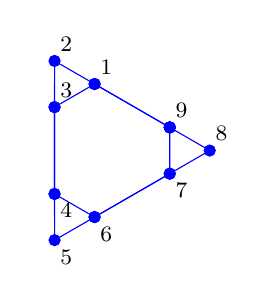
\begin{tikzpicture} 
\begin{axis}[footnotesize,font=\footnotesize
    ,axis equal image, axis lines=none ]
    \addplot[blue,mark=*,domain=40:400,samples=10
    ,nodes near coords={\quad\color{black}\ifnum\coordindex=0\else\coordindex\fi}] 
    ({cos(\x)+0.347*cos(2*\x)}
    ,{sin(\x)-0.347*sin(2*\x)});
    \addplot[blue,mark=*,samples at={40,80,160,200,280,320,40}] 
    ({cos(\x)+0.347*cos(2*\x)}
    ,{sin(\x)-0.347*sin(2*\x)});
\end{axis}
\end{tikzpicture}}%
\begin{equation*}
A=\begin{bmatrix}-3&1&1&0&0&0&0&0&1
\\1&-2&1&0&0&0&0&0&0
\\1&1&-3&1&0&0&0&0&0
\\0&0&1&-3&1&1&0&0&0
\\0&0&0&1&-2&1&0&0&0
\\0&0&0&1&1&-3&1&0&0
\\0&0&0&0&0&1&-3&1&1
\\0&0&0&0&0&0&1&-2&1
\\1&0&0&0&0&0&1&1&-3 \end{bmatrix}.
\end{equation*}
\begin{solution} 
In that example we used \script\ command \verb|[V,D]=eig(A)| to compute a matrix of eigenvectors~\verb|V| and the corresponding diagonal matrix of eigenvalues~\verb|D| where \twodp
{\small%??
\begin{verbatim}
V =
 -0.41  0.51 -0.16 -0.21 -0.45  0.18 -0.40  0.06  0.33
  0.00 -0.13  0.28  0.63  0.13 -0.18 -0.58 -0.08  0.33
  0.41 -0.20 -0.49 -0.42  0.32  0.01 -0.36 -0.17  0.33
 -0.41 -0.11  0.52 -0.42  0.32  0.01  0.14 -0.37  0.33
 -0.00 -0.18 -0.26  0.37 -0.22  0.51  0.36 -0.46  0.33
  0.41  0.53  0.07  0.05 -0.10 -0.51  0.33 -0.23  0.33
 -0.41 -0.39 -0.36  0.05 -0.10 -0.51  0.25  0.31  0.33
  0.00  0.31 -0.03  0.16  0.55  0.34  0.22  0.55  0.33
  0.41 -0.33  0.42 -0.21 -0.45  0.18  0.03  0.40  0.33
D =
 -5.00     0     0     0     0     0     0     0     0
     0 -4.30     0     0     0     0     0     0     0
     0     0 -4.30     0     0     0     0     0     0
     0     0     0 -3.00     0     0     0     0     0
     0     0     0     0 -3.00     0     0     0     0
     0     0     0     0     0 -3.00     0     0     0
     0     0     0     0     0     0 -0.70     0     0
     0     0     0     0     0     0     0 -0.70     0
     0     0     0     0     0     0     0     0 -0.00
\end{verbatim}
}%
%From these we identify the following eigenspaces:
%\begin{eqnarray*}
%&&\EE_{-5}=\Span\{(-1,0,1,-1,0,1,-1,0,1)\};
%\\&&\EE_{-4.30}=\Span\left\{ \begin{bmatrix} 0.51\\-0.13\\-0.20\\-0.11\\-0.18\\0.53\\-0.39\\0.31\\-0.33 \end{bmatrix},\  \begin{bmatrix} -0.16\\0.28\\-0.49\\0.52\\-0.26\\0.07\\-0.36\\-0.03\\0.42 \end{bmatrix} \right\};
%\\&&\EE_{-3}=\Span\left\{ 
%\begin{bmatrix} -0.21\\0.63\\-0.42\\-0.42\\0.37\\0.05\\0.05\\0.16\\-0.21
%\end{bmatrix},\  
%\begin{bmatrix} -0.45\\0.13\\0.32\\0.32\\-0.22\\-0.10\\-0.10\\0.55\\-0.45
%\end{bmatrix},\ 
%\begin{bmatrix} 0.18\\-0.18\\0.01\\0.01\\0.51\\-0.51\\-0.51\\0.34\\0.18
% \end{bmatrix} \right\};
%\\&&\EE_{-0.70}=\Span\left\{ \begin{bmatrix} -0.40\\-0.58\\-0.36\\0.14\\0.36\\0.33\\0.25\\0.22\\0.03 \end{bmatrix},\  \begin{bmatrix} 0.06\\-0.08\\-0.17\\-0.37\\-0.46\\-0.23\\0.31\\0.55\\0.40 \end{bmatrix} \right\}; 
%\\&&\EE_{0}=\Span\{(1,1,1,1,1,1,1,1,1)\}.
%\end{eqnarray*}
Since matrix~\(A\) is symmetric, \script\ computes for us an orthogonal matrix~\(V\) with columns eigenvectors.
Since~\(V\) is orthogonal its column vectors are orthonormal and hence its columns are linearly independent (\autoref{thm:ortholi}).
Since there exist nine linearly independent eigenvectors, the nine column vectors of~\(V\), the matrix~\(A\) is diagonalisable.
Further, the product \(V^{-1}AV=D\) for the above diagonal matrix~\(D\) of eigenvalues in the order of the eigenvectors in~\(V\).
(Also, since \(V\)~is orthogonal, \(\tr VAV=D\).)
\end{solution}
\end{example}





\begin{example} \label{eg:faespmp}
Recall \autoref{eg:faespm} found eigenvalues and corresponding eigenspaces for various matrices.
Revisit these cases and show none of the matrices are diagonalisable.
\begin{enumerate}
\item Matrix \(A=\begin{bmatrix} 3&1\\0&3 \end{bmatrix}\) had one eigenvalue \(\lambda=3\) with multiplicity two and corresponding eigenspace \(\EE_3=\Span\{(1,0)\}\).
This matrix is not diagonalisable as it has only one linearly independent eigenvector, such as~\((1,0)\) or any non-zero multiple, and it needs two. 

\item Matrix \(B=\begin{bmatrix}-1&1&-2
\\-1&0&-1
\\0&-3&1 \end{bmatrix}\)
has eigenvalues  \(\lambda=-2\) (multiplicity one) and \(\lambda=1\) (multiplicity two).
The corresponding eigenspaces are \(\EE_{-2}=\Span\{(1,1,1)\}\) and \(\EE_{1}=\Span\{(-1,0,1)\}\).
Thus the matrix has only two linearly independent eigenvectors, one from each eigenspace, and it needs three to be diagonalisable.

\item Matrix \(C=\begin{bmatrix}-1&0&-2
\\0&-3&2
\\0&-2&1\end{bmatrix}\)
has only the eigenvalue \(\lambda=-1\) with multiplicity three.
The corresponding eigenspace \(\EE_{-1}=\Span\{(1,0,0)\}\).
With only one linearly independent eigenvector, the matrix is not diagonalisable.

\end{enumerate}
\end{example}


\begin{example} \label{eg:fiveevp}
Use the results of \autoref{eg:fiveev} to show the following matrix is \idx{diagonalisable}:
\begin{equation*}
A=\begin{bmatrix}0&3&0&0&0
\\1&0&3&0&0
\\0&1&0&3&0
\\0&0&1&0&3
\\0&0&0&1&0\end{bmatrix}
\end{equation*}
\begin{solution} 
\autoref{eg:fiveev} derived the five eigenvalues are  \(\lambda=0,\pm\sqrt3,\pm3\)\,, all of multiplicity one.
Further, the corresponding eigenspaces are
\begin{eqnarray*}
&&\EE_0=\Span\{(9,0,-3,0,1)\},
\\&&\EE_{\pm\sqrt3}=\Span\{(-9,\mp3\sqrt3,0,\pm\sqrt3,1)\},
\\&&\EE_{\pm3}=\Span\{(9,\pm9,6,\pm3,1)\}.
\end{eqnarray*}
Here there are five linearly independent eigenvectors, one from each distinct eigenspace  (\autoref{thm:indepev}).
Since \(A\) is a \(5\times5\) matrix it is thus diagonalisable.
Further, \autoref{thm:gendiag} establishes that the matrix formed from the columns of the five eigenvectors will be a possible matrix
\begin{equation*}
P=\begin{bmatrix} 9&-9&-9&9&9
\\0&-3\sqrt3&3\sqrt3&9&-9
\\-3&0&0&6&6
\\0&\sqrt3&-\sqrt3&3&-3
\\1&1&1&1&1
\end{bmatrix}.
\end{equation*}
(One could also scale each column of~\(P\) by a different arbitrary non-zero constant, and the diagonalisation still holds.)
Lastly, \autoref{thm:gendiag} establishes the diagonal matrix
\(P^{-1}AP=D=\diag(0,\sqrt3,-\sqrt3,3,-3)\) is that of the eigenvalues in the order corresponding to the eigenvectors in~\(P\).
\end{solution}
\end{example}





These examples illustrate a widely useful property.
The \(5\times 5\) matrix in \autoref{eg:fiveevp} has five distinct eigenvalues whose corresponding eigenvectors are necessarily \idx{linearly independent} (\autoref{thm:indepev}) and so diagonalise the matrix (\autoref{thm:gendiag}).
The \(3\times 3\) matrix in \autoref{eg:trieigp} has three distinct eigenvalues whose corresponding eigenvectors are necessarily linearly independent (\autoref{thm:indepev}) and so diagonalise the matrix (\autoref{thm:gendiag}).
However, the matrices of Examples~\ref{eg:sier2eigp} and~\ref{eg:faespmp} have \idx{repeated eigenvalue}s---eigenvalues of \idx{multiplicity} two or more---and these matrices may (\autoref{eg:sier2eigp}) or may not (\autoref{eg:faespmp}) be diagonalisable.
The following theorem confirms that matrices with as many \emph{distinct} eigenvalues as the size of the matrix are always diagonalisable.






\begin{theorem} \label{thm:dlamd} 
For every \(n\times n\) \idx{square matrix}~\(A\), if~\(A\) has \(n\)~distinct \idx{eigenvalue}s, then \(A\)~is \idx{diagonalisable}.
Consequently, and allowing complex eigenvalues, a real \idx{non-diagonalisable matrix} must be non-symmetric and must have at least one \idx{repeated eigenvalue} (an eigenvalue with \idx{multiplicity} two or more).
\end{theorem}
\begin{proof}  
First, let \hlist\vv n\ be eigenvectors corresponding to the \(n\)~distinct eigenvalues of matrix~\(A\).
(Recall that \autoref{thm:geecp} establishes that there cannot be more than \(n\)~eigenvalues.)
As the corresponding eigenvalues are distinct, \autoref{thm:indepev} establishes that these eigenvectors are linearly independent.
\autoref{thm:gendiag} then establishes the matrix~\(A\) is diagonalisable.

Second, the converse of the first statement in the theorem then also holds.
Since an \(n\times n\) matrix has \(n\)~eigenvalues, when counted accordingly to multiplicity and allowing for complex eigenvalues (\autoref{pro:geneig}), a non-diagonalisable matrix must have at least one repeated eigenvalue.  
But further, by \autoref{thm:symspec} a real symmetric matrix is always diagonalisable: hence a non-diagonalisable matrix must also be non-symmetric.
\end{proof}


\begin{example} \label{eg:}
From the given information, are the matrices diagonalisable?
\begin{enumerate}
\item The only eigenvalues of a \(4\times 4\) matrix are \(1.8\), \(-3\), \(0.4\) and~\(3.2\).
\begin{solution} 
\autoref{thm:dlamd} implies the matrix must be diagonalisable.
\end{solution}

\item The only eigenvalues of a \(5\times 5\) matrix are \(1.8\), \(-3\), \(0.4\) and~\(3.2\).
\begin{solution} 
Here there are only four distinct eigenvalues of the \(5\times5\) matrix.
\autoref{thm:dlamd} does not apply as the precondition that there be five distinct eigenvalues is not met: the matrix may or may not be diagonalisable---it is unknowable on this information.
\end{solution}

\item The only eigenvalues of a \(3\times 3\) matrix are \(1.8\), \(-3\), \(0.4\) and~\(3.2\).
\begin{solution} 
An error has been made in determining the eigenvalues as a \(3\times3\) matrix has at most three distinct eigenvalues (\autoref{thm:geecp}).
Because of the error, we cannot answer.
\end{solution}

\end{enumerate}
\end{example}



\begin{activity}
A \(3\times3\) matrix~\(A\) depends upon a parameter~\(a\) and has eigenvalues \(6\), \(3-3a\) and \(2+a\)\,.
For which of the following values of parameter~\(a\) may the matrix be \emph{not} diagonalisable?
\actposs[4]{\(a=4\)}{\(a=1\)}{\(a=2\)}{\(a=3\)}
%\partswidth=5em
%\begin{parts}
%\item \(a=1\)
%\item \(a=2\)
%\item \(a=3\)
%\item \(a=4\)\actans
%\end{parts}
\end{activity}





\begin{example} \label{eg:}
\script\ computes the eigenvalues of matrix
\begin{equation*}
A=\begin{bmatrix}-1&2&-2&1&-2
\\-3&-1&-2&5&6
\\3&1&6&-2&-1
\\1&1&2&1&-1
\\7&5&-3&0&0 \end{bmatrix}
\end{equation*}
via \verb|eig(A)| and reports them to be \twodp
\begin{verbatim}
ans =
  -3.45 + 3.50i
  -3.45 - 3.50i
   5.00
   5.00
   1.91
\end{verbatim}
Is the matrix diagonalisable?
\begin{solution} 
The matrix appears to have only four distinct eigenvalues (two of them complex valued), and so on the given information \autoref{thm:dlamd} cannot determine whether the matrix is diagonalisable or not.

However, upon reporting the eigenvalues to four decimal places we find the two eigenvalues of~\verb|5.00| \twodp\ are more precisely two separate eigenvalues of~\verb|5.0000| and~\verb|4.9961|.
Hence this matrix has five distinct eigenvalues and so \autoref{thm:dlamd} implies the matrix is diagonalisable.
\footnote{Nonetheless, in an application where errors are significant then the matrix may be effectively non-diagonalisable.
Such effective non-diagonalisability is indicated by poor conditioning of the matrix of eigenvectors which here has the poor \texttt{rcond} of~\(0.0004\) (\autoref{pro:unisol}).}
\end{solution}
%\begin{verbatim}
%for i=1:99999,a=round(randn(5)*3); if abs(min(abs(diff(eig(a))))-3e-3)<2e-3, eig(a), break, end, end
%\end{verbatim}
\end{example}






Recall that for every \idx{symmetric matrix}, from \autoref{def:eigsymult}, the dimension of an eigenspace,~\(\dim\EE_{\lambda_j}\) is equal to the multiplicity of the corresponding eigenvalue~\(\lambda_j\).
However, for general matrices this equality is not necessarily so.


\begin{theorem} \label{thm:dimee} 
For every square matrix~\(A\), and for each \idx{eigenvalue}~\(\lambda_j\) of~\(A\), the corresponding \idx{eigenspace}~\(\EE_{\lambda_j}\) has \idx{dimension} less than or equal to the \idx{multiplicity} of~\(\lambda_j\);
that is, \(1\leq\dim\EE_{\lambda_j}\leq\text{multiplicity of }\lambda_j\)\,.  
\end{theorem}
%\begin{comment}
%Maths I 2014 course omits any proof.
%\end{comment}
%\begin{proof} 
%Suppose \(\lambda_j\) is an eigenvalue of matrix~\(A\) and \(\dim\EE_{\lambda_j}=p<n\) (the case \(p=n\) is proved by \autoref{ex:dimme}).
%Then to span \(\EE_{\lambda_j}\) there are \(p\) corresponding, linearly independent, eigenvectors \hlist\vv p\,.
%Let
%\begin{equation*}
%P=\begin{bmatrix} \vv_1&\cdots&\vv_p&\wv_{p+1}&\cdots&\wv_n \end{bmatrix}
%\end{equation*}
%be any invertible matrix with \hlist\vv p\ as its first \(p\)~columns.
%Equivalently, write as the partitioned matrix \(P=\begin{bmatrix} V&W \end{bmatrix}\) for corresponding \(n\times p\) and \(n\times(n-p)\) matrices.
%Since the columns of~\(V\) are eigenvectors corresponding to eigenvalue~\(\lambda_j\), \(AV=A\begin{bmatrix} \vv_1&\cdots&\vv_p \end{bmatrix}
%=\begin{bmatrix} A\vv_1&\cdots&A\vv_p \end{bmatrix}
%=\begin{bmatrix} \lambda_j\vv_1&\cdots&\lambda_j\vv_p \end{bmatrix}
%=\lambda_j\begin{bmatrix} \vv_1&\cdots&\vv_p \end{bmatrix}
%=\lambda_jV\).
%Partition the inverse of~\(P\) as \(P^{-1}=\begin{bmatrix} B\\C \end{bmatrix}\) for \(p\times n\) and \((n-p)\times n\) matrices~\(B\) and~\(C\), respectively.
%From this partitioning,
%\begin{eqnarray*}&&
%P^{-1}P=\begin{bmatrix} B\\C \end{bmatrix}\begin{bmatrix} V&W \end{bmatrix}
%=\begin{bmatrix} BV&BW\\CV&CW \end{bmatrix}
%\\\text{and}&&
%P^{-1}P=I_n=\begin{bmatrix} I_p&O\\O&I_{n-p} \end{bmatrix},
%\end{eqnarray*}
%so \(BV=I_p\)\,, \(BW=O\)\,, \(CV=O\) and \(CW=I_{n-p}\)\,.
%
%Now consider
%\begin{eqnarray*}
%P^{-1}AP
%&=&\begin{bmatrix} B\\C \end{bmatrix}A\begin{bmatrix} V&W \end{bmatrix}
%=\begin{bmatrix} BAV&BAW\\CAV&CAW \end{bmatrix}
%\\
%&=&\begin{bmatrix} \lambda_jBV&BAW\\\lambda_jCV&CAW \end{bmatrix}
%=\begin{bmatrix} \lambda_jI_p&BAW\\O&CAW \end{bmatrix}
%\end{eqnarray*}
%Then the characteristic polynomial of matrix~\(A\) becomes
%\begin{eqnarray*}
%&&\hspace{-1.5em}\det(A-\lambda I_n)
%\\&=&\det(PP^{-1}APP^{-1}-\lambda PP^{-1})
%\quad(\text{as }PP^{-1}=I_n)
%\\&=&\det[P(P^{-1}AP-\lambda I_n)P^{-1}]
%\\&=&\det P\det(P^{-1}AP-\lambda I_n)\det(P^{-1})
%\quad(\text{product Thm.~\ref{thm:detprod}})
%\\&=&\det P\det(P^{-1}AP-\lambda I_n)\frac1{\det P}
%\quad(\text{inverse Thm.~\ref{thm:detinv}})
%\\&=&\det(P^{-1}AP-\lambda I_n)
%\\&=&\det\begin{bmatrix} (\lambda_j-\lambda)I_p&BAW\\O&CAW -\lambda I_{n-p}\end{bmatrix}
%\quad(\text{by above }PAP^{-1})
%\\&=&(\lambda_j-\lambda)^p\det(CAW -\lambda I_{n-p})
%\end{eqnarray*}
%by \(p\)~successive first column expansions of the determinant (\autoref{thm:letdet}).
%Because of the factor \((\lambda_j-\lambda)^p\) in the characteristic polynomial of~\(A\), the eigenvalue~\(\lambda_j\) must have multiplicity of at least~\(p=\dim\EE_{\lambda_j}\)
%(there may be more factors of \((\lambda_j-\lambda)\) hidden within \(\det(CAW -\lambda I_{n-p})\)).
%\end{proof}
\begin{proof} 
Suppose \(\lambda_j\) is an eigenvalue of matrix~\(A\) and \(\dim\EE_{\lambda_j}=p<n\) (the case \(p=n\) is proved by \autoref{ex:dimme}).
Because its dimension is~\(p\) the eigenspace may be spanned by \(p\)~vectors.
Then choose \(p\)~orthonormal vectors \hlist\vv p\ to span~\(\EE_{\lambda_j}\): these vectors \hlist\vv p\ are eigenvectors as they are in the eigenspace.
Let
\begin{equation*}
P=\begin{bmatrix} \vv_1&\cdots&\vv_p&\wv_{p+1}&\cdots&\wv_n \end{bmatrix}
\end{equation*}
be any orthogonal matrix with \hlist\vv p\ as its first \(p\)~columns.
Equivalently, write as the partitioned matrix \(P=\begin{bmatrix} V&W \end{bmatrix}\) for corresponding \(n\times p\) and \(n\times(n-p)\) matrices.
Since \(P\)~is orthogonal, its inverse \(P^{-1}=\tr P=\begin{bmatrix} \tr V\\\tr W \end{bmatrix}\).
Since the columns of~\(V\) are eigenvectors corresponding to eigenvalue~\(\lambda_j\), \(AV=A\begin{bmatrix} \vv_1&\cdots&\vv_p \end{bmatrix}
=\begin{bmatrix} A\vv_1&\cdots&A\vv_p \end{bmatrix}
=\begin{bmatrix} \lambda_j\vv_1&\cdots&\lambda_j\vv_p \end{bmatrix}
=\lambda_j\begin{bmatrix} \vv_1&\cdots&\vv_p \end{bmatrix}
=\lambda_jV\).

Now consider
\begin{eqnarray*}
P^{-1}AP
&=&\begin{bmatrix} \tr V\\\tr W \end{bmatrix}A\begin{bmatrix} V&W \end{bmatrix}
=\begin{bmatrix} \tr VAV&\tr VAW\\\tr WAV&\tr WAW \end{bmatrix}
\\
&=&\begin{bmatrix} \lambda_j\tr VV&\tr VAW\\\lambda_j\tr WV&\tr WAW \end{bmatrix}
=\begin{bmatrix} \lambda_jI_p&\tr VAW\\O&\tr WAW \end{bmatrix}
\end{eqnarray*}
where the last equality follows from the orthonormality of columns of \(P=\begin{bmatrix} V&W \end{bmatrix}\).
Then the characteristic polynomial of matrix~\(A\) becomes
\begin{eqnarray*}
&&\hspace{-1.5em}\det(A-\lambda I_n)
\\&=&\det(PP^{-1}APP^{-1}-\lambda PP^{-1})
\quad(\text{as }PP^{-1}=I_n)
\\&=&\det[P(P^{-1}AP-\lambda I_n)P^{-1}]
\\&=&\det P\det(P^{-1}AP-\lambda I_n)\det(P^{-1})
\quad(\text{product Thm.~\ref{thm:detprod}})
\\&=&\det P\det(P^{-1}AP-\lambda I_n)\frac1{\det P}
\quad(\text{inverse Thm.~\ref{thm:detinv}})
\\&=&\det(P^{-1}AP-\lambda I_n)
\\&=&\det\begin{bmatrix} (\lambda_j-\lambda)I_p&\tr VAW\\O&\tr WAW -\lambda I_{n-p}\end{bmatrix}
\quad(\text{by above }P^{-1}AP)
\\&=&(\lambda_j-\lambda)^p\det(\tr WAW -\lambda I_{n-p})
\end{eqnarray*}
by \(p\)~successive first column expansions of the determinant (\autoref{thm:letdet}).
Because of the factor \((\lambda_j-\lambda)^p\) in the characteristic polynomial of~\(A\), the eigenvalue~\(\lambda_j\) must have multiplicity of at least~\(p=\dim\EE_{\lambda_j}\)
---there may be more factors of \((\lambda_j-\lambda)\) hidden within \(\det(\tr WAW -\lambda I_{n-p})\).
\end{proof}



\begin{example} \label{eg:}
Show the following matrix has one eigenvalue of multiplicity three, and the corresponding eigenspace has dimension two:
\begin{equation*}
A=\begin{bmatrix}0&5&6
\\-8&22&24
\\6&-15&-16 \end{bmatrix}
\end{equation*}
\begin{solution} 
Find eigenvalues via the characteristic polynomial
\begin{eqnarray*}
\det(A-\lambda I)
&=&
\begin{vmatrix} -\lambda&5&6
\\-8&22-\lambda&24
\\6&-15&-16-\lambda \end{vmatrix}
\\&=&-\lambda(22-\lambda)(-16-\lambda)+5\cdot24\cdot6+6(-8)(-15)
\\&&{}-6(22-\lambda)6+\lambda24(-15)-5(-8)(-16-\lambda)
\\&=&\cdots
\\&=&-\lambda^3+6\lambda^2-12\lambda+8
\\&=&-(\lambda-2)^3.
\end{eqnarray*}
This characteristic polynomial is zero only for eigenvalue \(\lambda=2\) which is of multiplicity three.

The corresponding eigenspace comes from solving \((A-\lambda I)\xv=\ov\) which here is
\begin{equation*}
\begin{bmatrix}-2&5&6
\\-8&20&24
\\6&-15&-18 \end{bmatrix}\xv=\ov.
\end{equation*}
Observe that the second row is just four times the first row, and the third row is \((-3)\times{}\)the first row, hence all three equations in this system are equivalent to just the one from the first row, namely \(-2x_1+5x_2+6x_3=0\)\,.
A general solution of this equation is \(x_1=\tfrac52x_2-3x_3\)\,.
That is all solutions are \(\xv=(\tfrac52x_2-3x_3,x_2,x_3)=x_2(\tfrac52,1,0)+x_3(-3,0,1)\). 
Hence all solutions form the two dimensional eigenspace 
\(\EE_2=\Span\{(\tfrac52,1,0)\), \((-3,0,1)\}\).
\end{solution}
\end{example}



\begin{example} \label{eg:}
Use \script\ to find the eigenvalues and the dimension of the eigenspaces of the matrix 
\begin{equation*}
B=\begin{bmatrix} 344&-1165&-149&-1031&1065&-2816
\\90&-306&-38&-272&280&-742
\\-45&140&12&117&-115&302
\\135&-470&-70&-421&445&-1175
\\-165&555&67&493&-506&1338
\\-105&360&48&322&-335&886 \end{bmatrix}.
\end{equation*}

\begin{solution} 
In \script\ enter the matrix with
\begin{verbatim}
B=[344 -1165  -149 -1031  1065 -2816
    90  -306   -38  -272   280  -742
   -45   140    12   117  -115   302
   135  -470   -70  -421   445 -1175
  -165   555    67   493  -506  1338
  -105   360    48   322  -335   886]
\end{verbatim}
\setbox\ajrqrbox\hbox{\qrcode{% eigenspaces
B=[344 -1165  -149 -1031  1065 -2816
    90  -306   -38  -272   280  -742
   -45   140    12   117  -115   302
   135  -470   -70  -421   445 -1175
  -165   555    67   493  -506  1338
  -105   360    48   322  -335   886]
[V,D]=eig(B)
svd(V(:,1:3))
svd(V(:,4:6))
}}%
\marginpar{\usebox{\ajrqrbox}}%
Then \verb|[V,D]=eig(B)| computes something like the following \twodp
\begin{verbatim}
V =
  -0.19   0.19  -0.45   0.75  -0.20   0.15
  -0.38   0.38   0.12   0.26  -0.03   0.00
  -0.58   0.58   0.08  -0.00  -0.54   0.56
  -0.00  -0.00  -0.83   0.28  -0.50   0.52
   0.58  -0.58  -0.29  -0.45  -0.64   0.63
   0.38  -0.38   0.08  -0.29  -0.04   0.03
D =
   4.00      0      0      0      0      0
      0   4.00      0      0      0      0
      0      0   4.00      0      0      0
      0      0      0  -1.00      0      0
      0      0      0      0  -1.00      0
      0      0      0      0      0  -1.00
\end{verbatim}
Evidently, the matrix~\(B\) has two eigenvalues, \(\lambda=4\) and \(\lambda=-1\)\,, both of multiplicity three (although due to round-off error \script\ will report these with errors of about~\(10^{-5}\) (\autoref{sec:reas})---possibly complex errors in which case ignore small complex parts).
For each eigenvalue \script\ reports, the three corresponding columns of~\verb|V| contain corresponding eigenvectors.
Each set of these three eigenvectors do span the corresponding eigenspace, but are not necessarily linearly independent.
\begin{itemize}
\item For eigenvalue \(\lambda=4\) the first two columns of~\verb|V| are clearly the negative of each other, and so are essentially the same eigenvector.  
The third column of~\verb|V| is clearly not proportional to the first two columns and so is linearly independent (\autoref{thm:lindeplc}).
Thus \script\ has computed only two linearly independent eigenvectors, either the first and third column, or the second and third column.
Consequently, the dimension \(\dim\EE_4=2\)\,.

One can confirm this dimensionality by computing the singular values of the first three columns of~\verb|V| with \verb|svd(V(:,1:3))| to find they are \(1.4278\), \(0.9806\) and \(0.0000\).
The two non-zero singular values indicate the dimension of the span is two (\autoref{pro:ospan}).

\item For eigenvalue \(\lambda=-1\) the last three columns of~\verb|V| look linearly independent and so we suspect the eigenspace dimension \(\dim\EE_{-1}=3\)\,.

%If the dimensionality of an eigenspace is less than the multiplicity of an eigenvalue, then \script\ generally computes two columns as the same or the negative of each other (as for \(\lambda=-4\) here), so that the lower dimensionality is clearly apparent.
%However, this computed result is not guaranteed.
To confirm the dimension of this eigenspace via \autoref{pro:ospan}, compute \verb|svd(V(:,4:6))| to find the three singular values are \(1.4136\), \(1.0001\) and \(0.0414\).
Since all three singular values are non-zero, \(\dim\EE_{-1}=3\)\,.
\end{itemize}
\end{solution}
%\begin{verbatim}
%d=diag([-1 -1 -1 4 4 4]);
%d(4,5)=1;%d(5,6)=1;;
%for i=1:999999,p=round(randn(6)*3); if min(abs(abs(det(p))-[1 2 5]))<1e-7, a=p*d*inv(p), break, end, end
%\end{verbatim}
\script\ may produce for you a quite different matrix~\verb|V| of eigenvectors (possibly with complex parts). 
As discussed by \autoref{sec:reas}, repeated eigenvalues are very sensitive and this sensitivity means small variations in the hidden \script\ algorithm may produce quite large changes in the matrix~\verb|V| for repeated eigenvalues.
However, each eigenspace spanned by the appropriate columns of~\verb|V| is robust.
\end{example}





\subsection{Solve systems of differential equations}
\label{sec:ssde}
\index{differential equations|(}

\paragraph{Population modelling}
The population modelling seen so far (\autoref{sec:ddp}) expressed the changes of the population over discrete intervals in time via discrete time equations such as \(y(t+1)=\cdots\) and \(z(t+1)=\cdots\)\,.
One such example is to describe the population numbers year by year.
The alternative is to model the changes in the population \emph{continuously} in time.
This alternative invokes and analyses differential equations.
Such continuous time, differential equation, models are common for exploring the interaction between different species, such as humans and viruses.

Let's start with a continuous time version of the population modelling discussed at the start of this \autoref{ch:gee}.
Let two species interact continuously in time with populations \(y(t)\) and~\(z(t)\) at time~\(t\) (years).
Suppose they interact according to \idx{differential equation}s \(dy/dt=y-4z\) and \(dz/dt=-y+z\) (instead of the discrete time equations \(y(t+1)=\cdots\) and \(z(t+1)=\cdots\)).
Analogous to the start of this \autoref{sec:dit}, we now ask the following question: is there a matrix transformation to new variables, the vector~\(\Yv(t)\), such that \((y,z)=P\Yv\) for some as yet unknown matrix~\(P\), where the differential equations for~\Yv\ are simple?
\begin{itemize}
\item First, form the differential equations into a matrix-vector system:
\begin{equation*}
\begin{bmatrix} dy/dt\\dz/dt \end{bmatrix}
=\begin{bmatrix} y-4z
\\ -y+z \end{bmatrix}
=\begin{bmatrix} 1&-4\\-1& 1 \end{bmatrix}\begin{bmatrix} y\\z \end{bmatrix}.
\end{equation*}
So using vector \(\yv=(y,z)\), this system is
\begin{equation*}
\D t\yv=A\yv
\quad\text{for matrix }A=\begin{bmatrix} 1&-4\\-1& 1 \end{bmatrix}.
\end{equation*}

\item Second, see what happens when we transform to some, as yet unknown, new variables~\(\Yv(t)\) such that \(\yv=P\Yv\) for some constant invertible matrix~\(P\).
Under such a transform: \(\D t\yv=\D t{}P\Yv=P\D t\Yv\); also \(A\yv=AP\Yv\).
Hence substituting such an assumed transformation into the differential equations leads to
\begin{equation*}
P\D t\Yv=AP\Yv\,, 
\quad\text{that is}\quad
\D t\Yv=\left(P^{-1}AP\right)\Yv.
\end{equation*}
To simplify this system for~\Yv, we diagonalise the matrix on the right-hand side.
The procedure is to choose the columns of~\(P\) to be eigenvectors of the matrix~\(A\) (\autoref{thm:gendiag}).

\item Third, find the eigenvectors of~\(A\) by hand as it is a \(2\times2\) matrix. 
Here the matrix \(A=\begin{bmatrix} 1&-4\\-1&1 \end{bmatrix}\) has characteristic polynomial \(\det(A-\lambda I)=(1-\lambda)^2-4\)\,.
This is zero for \((1-\lambda)^2=4\)\,, that is, \((1-\lambda)=\pm2\).
Hence the eigenvalues \(\lambda=1\pm2=3,-1\)\,.
\begin{itemize}
\item For eigenvalue \(\lambda_1=3\) the corresponding eigenvectors satisfy
\begin{equation*}
(A-\lambda_1I)\pv_1=\begin{bmatrix} -2&-4\\-1&-2 \end{bmatrix}\pv_1=\ov\,,
\end{equation*}
with general solution \(\pv_1\propto(2,-1)\).

\item For eigenvalue \(\lambda_2=-1\) the corresponding eigenvectors satisfy
\begin{equation*}
(A-\lambda_2I)\pv_2=\begin{bmatrix} 2&-4\\-1&2 \end{bmatrix}\pv_2=\ov\,,
\end{equation*}
with general solution \(\pv_2\propto(2,1)\).
\end{itemize}
Thus setting transformation matrix 
\begin{equation*}
P=\begin{bmatrix} 2&2\\-1&1 \end{bmatrix}
\implies \D t\Yv=\begin{bmatrix} 3&0\\0&-1 \end{bmatrix}\Yv
\end{equation*}
(any scalar multiple of the two columns of~\(P\) would also work).

\item Fourth, having diagonalised the matrix, expand this diagonalised set of differential equations to write this system in terms of components: 
\begin{equation*}
\D t{Y_1}=3Y_1 \quad\text{and}\quad \D t{Y_2}=-Y_2\,.
\end{equation*}
Each of these differential equations have well-known exponential solutions, respectively \(Y_1=c_1e^{3t}\) and \(Y_2=c_2e^{-t}\),  for every constants~\(c_1\) and~\(c_2\).

\item Lastly, what does this mean for the original problem?
From the relation
\begin{equation*}
\begin{bmatrix} y\\z \end{bmatrix}=\yv
=P\Yv=\begin{bmatrix} 2&2\\-1&1 \end{bmatrix}
\begin{bmatrix}c_1e^{3t}\\ c_2e^{-t} \end{bmatrix}
=\begin{bmatrix} 2c_1e^{3t}+2c_2e^{-t}
\\ -c_1e^{3t}+c_2e^{-t}\end{bmatrix}.
\end{equation*}
That is, a general solution of the original system of differential equations is \(y(t)=2c_1e^{3t}+2c_2e^{-t}\) and \(z(t)=-c_1e^{3t}+c_2e^{-t}\).

\end{itemize}
The diagonalisation of the matrix empowers us to solve complicated systems of differential equations as a set of simple systems.


Such a \idx{general solution} makes predictions. 
For example, suppose at time zero (\(t=0\)) the initial population of female \(y\)-animals is~\(22\) and the population of female \(z\)-animals is~\(9\).
From the above general solution we then know that at time \(t=0\)
\begin{equation*}
\begin{bmatrix} 22\\9 \end{bmatrix}=
\begin{bmatrix} y(0)\\z(0) \end{bmatrix}
=\begin{bmatrix} 2c_1e^{3\cdot0}+2c_2e^{-0}
\\ -c_1e^{3\cdot0}+c_2e^{-0} \end{bmatrix}
=\begin{bmatrix} 2c_1+2c_2
\\ -c_1+c_2 \end{bmatrix}
\end{equation*}
This determines the coefficients: \(2c_1+2c_2=22\)
and \(-c_1+c_2=9\)\,.
Adding the first to twice the second gives \(4c_2=40\)\,, that is, \(c_2=10\)\,.
Then either equation determines \(c_1=1\)\,.
Consequently, the \idx{particular solution} from this initial population is
\begin{equation*}
\begin{bmatrix} y\\z \end{bmatrix}
=\begin{bmatrix} 2\cdot1e^{3t}+2\cdot10e^{-t}
\\ -1e^{3t}+10e^{-t}\end{bmatrix}
=\begin{bmatrix} 2e^{3t}+20e^{-t}
\\ -e^{3t}+10e^{-t}\end{bmatrix}.
\end{equation*}
\begin{center}
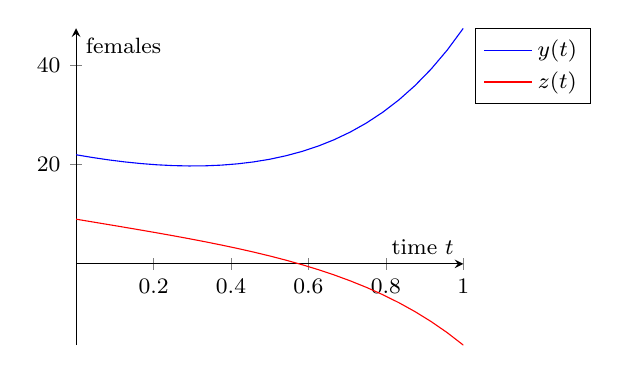
\begin{tikzpicture}
\begin{axis}[small,font=\footnotesize,domain=0:1, 
xlabel={time $t$},ylabel={females},axis lines=middle
,legend pos=outer north east]
\addplot [blue] {2*exp(3*x)+20*exp(-x)};
\addlegendentry{$y(t)$};
\addplot [red] {-exp(3*x)+10*exp(-x)};
\addlegendentry{$z(t)$};
\end{axis}
\end{tikzpicture}
\end{center}
The above graph of this solution shows that the population of \(y\)-animals grows in time, whereas the population of \(z\)-animals crashes and becomes extinct at about time \(0.6\)~years.%
\footnote{After time \(0.6\)~years the differential equation model  and its predictions becomes meaningless as there is no biological meaning to a negative number of animals~\(z\).}


The forthcoming \autoref{thm:ddtsol} confirms that the same approach solves general systems of differential equations: it corresponds to \autoref{thm:dynsol} for discrete dynamics.



\begin{activity}
A given population model is expressed as the differential equations \(dx/dt=x+y-3z\)\,, \(dy/dt=-2x+z\) and \(dz/dt=-2x+y+2z\)\,.
This may be written in matrix-vector form \(d\xv/dt=A\xv\) for vector \(\xv(t)=(x,y,z)\) and which of the following matrices?
\actposs{\(\begin{bmatrix} 1&1&-3
\\-2&0&1
\\-2&1&2 \end{bmatrix}\)}
{\(\begin{bmatrix} 1&-3&1
\\-2&1&0
\\-2&2&1 \end{bmatrix}\)}
{\(\begin{bmatrix} 1&-2&2
\\0&-2&1
\\1&1&-3 \end{bmatrix}\)}
{\(\begin{bmatrix} 1&1&-3
\\0&-2&1
\\1&-2&2 \end{bmatrix}\)}
%\begin{parts}
%\item \(\begin{bmatrix} 1&-3&1
%\\-2&1&0
%\\-2&2&1 \end{bmatrix}\)
%\item \(\begin{bmatrix} 1&-2&2
%\\0&-2&1
%\\1&1&-3 \end{bmatrix}\)
%\item\actans \(\begin{bmatrix} 1&1&-3
%\\-2&0&1
%\\-2&1&2 \end{bmatrix}\)
%\item \(\begin{bmatrix} 1&1&-3
%\\0&-2&1
%\\1&-2&2 \end{bmatrix}\)
%\end{parts}
\end{activity}




\begin{theorem} \label{thm:ddtsol}
Let \(n\times n\) \idx{square matrix}~\(A\) be \idx{diagonalisable} by matrix \(P=\begin{bmatrix} \pv_1&\pv_2&\cdots&\pv_n \end{bmatrix}\) whose columns are \idx{eigenvector}s corresponding to \idx{eigenvalue}s \hlist\lambda n.  
Then a \idx{general solution}~\(\xv(t)\) to the \idx{differential equation} system \(d\xv/dt=A\xv\) is the \idx{linear combination}
\begin{equation}
\xv(t)=c_1\pv_1e^{\lambda_1t}+c_2\pv_2e^{\lambda_2t}+\cdots+c_n\pv_ne^{\lambda_nt}
\label{eq:ddtsol}
\end{equation}
for arbitrary constants \hlist cn.
\end{theorem}

\begin{proof} 
First, instead of finding solutions for~\(\xv(t)\) directly, let's write the differential equations in terms of the alternate basis for~\(\RR^n\), basis \(\cP=\{\hlist\pv n\}\) (as \hlist\pv n\ are linearly independent).
That is, solve for the coordinates \(\Xv(t)=[\xv(t)]_\cP\) with respect to basis~\cP.
Now recall (\autoref{thm:ssbc}) that  \(\Xv=[\xv]_\cP\) means that \(\xv=\lincomb X\pv n=P\Xv\)\,.
Substitute this into the differential equation \(d\xv/dt=A\xv\) requires \(\D t{}(P\Xv)=A(P\Xv)\) which is the same as \(P\D t\Xv=AP\Xv\)\,.
Since matrix~\(P\) is invertible, this equation is the same as \(\D t\Xv=P^{-1}AP\Xv\)\,.
Because the columns of matrix~\(P\) are eigenvectors, the product \(P^{-1}AP\) is the diagonal matrix \(D=\diag(\hlist\lambda n)\), hence the system becomes \(\D t\Xv=D\Xv\)\,.
Because matrix~\(D\) is diagonal, this is a much simpler system of differential equations.
The \(n\)~rows of the system are
\begin{equation*}
\D t{X_1}=\lambda_1X_1\,,\quad
\D t{X_2}=\lambda_2X_2\,,\quad \ldots,\quad
\D t{X_n}=\lambda_nX_n\,.
\end{equation*}
Each of these have general solution
\begin{equation*}
X_1=c_1e^{\lambda_1t},\quad
X_2=c_2e^{\lambda_2t},\quad \ldots,\quad
X_n=c_ne^{\lambda_nt},
\end{equation*}
where \hlist cn\ are arbitrary constants.
To rewrite this solution for the original coordinates~\xv\ use
\begin{eqnarray*}
\xv&=&P\Xv
\\&=&\begin{bmatrix} \pv_1&\pv_2&\cdots&\pv_n \end{bmatrix}
\begin{bmatrix} c_1e^{\lambda_1t}
\\c_2e^{\lambda_2t}
\\\vdots
\\c_ne^{\lambda_nt} \end{bmatrix}
\\&=&c_1\pv_1e^{\lambda_1t}+c_2\pv_2e^{\lambda_2t}+\cdots+c_n\pv_ne^{\lambda_nt}
\end{eqnarray*}
to derive the solution~\eqref{eq:ddtsol}.

\begin{comment}
Straightforward substitution is simpler, but the above reinforces the simplification through diagonalisation.
\end{comment}
%First show that formula~\eqref{eq:ddtsol} is a solution by substitution into the differential equation \(d\xv/dt=A\xv\)\,: recalling from calculus that \(\D t{}e^{at}=ae^{at}\), the left-hand side
%\begin{eqnarray*}
%\D t\xv&=&c_1\pv_1\D t{}e^{\lambda_1t}+c_2\pv_2\D t{}e^{\lambda_2t}+\cdots+c_n\pv_n\D t{}e^{\lambda_nt}
%\\&=&c_1\pv_1\lambda_1e^{\lambda_1t}+c_2\pv_2\lambda_2e^{\lambda_2t}+\cdots+c_n\pv_n\lambda_ne^{\lambda_nt}\,;
%\end{eqnarray*}
%whereas the right-hand side, as \(\pv_j\) are eigenvectors,
%\begin{eqnarray*}
%A\xv&=&c_1A\pv_1e^{\lambda_1t}+c_2A\pv_2e^{\lambda_2t}+\cdots+c_nA\pv_ne^{\lambda_nt}
%\\&=&c_1\lambda_1\pv_1e^{\lambda_1t}+c_2\lambda_2\pv_2e^{\lambda_2t}+\cdots+c_n\lambda_n\pv_ne^{\lambda_nt}.
%\end{eqnarray*}
%These expressions are the same and hence formula~\eqref{eq:ddtsol} solves \(d\xv/dt=A\xv\)\,.

Second, being able to use the constants \(\cv=(\hlist cn)\) to match every given initial condition shows formula~\eqref{eq:ddtsol} is a general solution.
Suppose the value of~\(\xv(0)\) is given.
Recalling \(e^0=1\)\,, formula~\eqref{eq:ddtsol} evaluated at \(t=0\)  requires
\begin{eqnarray*}
\xv(0)&=&c_1\pv_1e^{\lambda_10}+c_2\pv_2e^{\lambda_20}+\cdots+c_n\pv_ne^{\lambda_n0}
\\&=&c_1\pv_1+c_2\pv_2+\cdots+c_n\pv_n
\\&=&\begin{bmatrix} \pv_1&\pv_2&\cdots&\pv_n \end{bmatrix}\cv
\\&=&P\cv\,.
\end{eqnarray*}
Since matrix~\(P\) is invertible, choose constants \(\cv=P^{-1}\xv(0)\) for any given~\(\xv(0)\).
%Theorems~\ref{thm:gendiag} and~\ref{thm:ftim3} establish that such an invertible~\(P\) exists for diagonalisable matrices~\(A\).
\end{proof}





\begin{activity}
Recall that the \idx{differential equation}s \(dy/dt=y-4z\) and \(dz/dt=-y+z\) have a \idx{general solution} \(y(t)=2c_1e^{3t}+2c_2e^{-t}\) and \(z(t)=-c_1e^{3t}+c_2e^{-t}\).
What are the values of these constants given that \(y(0)=2\) and \(z(0)=3\)?
\actposs{\(c_1=-1\), \(c_2=2\)}
{\(c_1=c_2=1\)}
{\(c_1=0\), \(c_2=-1\)}
{\(c_1=-2\), \(c_2=0\)}
%\begin{parts}
%\item \(c_1=c_2=1\)
%\item \(c_1=0\), \(c_2=-1\)
%\item \(c_1=-2\), \(c_2=0\)
%\item\actans \(c_1=-1\), \(c_2=2\)
%\end{parts}
\end{activity}




\begin{example} \label{eg:de3t} 
Find (by hand) a general solution to the system of differential equations \(\D tu=-2u+2v\)\,, \(\D tv=u-2v+w\)\,, and \(\D tw=2v-2w\)\,.

\begin{solution} 
Let vector~\(\uv=(u,v,w)\), and then form the differential equations into the matrix-vector system
\begin{eqnarray*}
\D t\uv&=&\begin{bmatrix} \D tu\\\D tv\\\D t w \end{bmatrix}
=\begin{bmatrix} -2u+2v\\u-2v+w\\2v-2w \end{bmatrix}
\\&=&\begin{bmatrix} -2&2&0\\1&-2&1\\0&2&-2 \end{bmatrix}
\begin{bmatrix} u\\v\\w \end{bmatrix}
=\underbrace{\begin{bmatrix} -2&2&0\\1&-2&1\\0&2&-2 \end{bmatrix}}_A\uv\,.
\end{eqnarray*}
To use \autoref{thm:ddtsol} we need eigenvalues and eigenvectors of the matrix~\(A\).
Here the characteristic polynomial of~\(A\) is, using~\eqref{eq:dets23b},
\begin{eqnarray*}
\det(A-\lambda I)&=&\det\begin{bmatrix} -2-\lambda&2&0\\1&-2-\lambda&1\\0&2&-2-\lambda \end{bmatrix}
\\&=&-(2+\lambda)^3+0+0-0+2(2+\lambda)+2(2+\lambda)
\\&=&(2+\lambda)\left[-(2+\lambda)^2+4\right]
\\&=&(2+\lambda)[-\lambda^2-4\lambda]
\\&=&-\lambda(\lambda+2)(\lambda+4).
\end{eqnarray*}
This determinant is only zero for eigenvalues \(\lambda=0,-2,-4\)\,.
\begin{itemize}
\item For eigenvalue \(\lambda=0\)\,, corresponding eigenvectors~\pv\ satisfy
\begin{equation*}
(A-0I)\pv=\begin{bmatrix} -2&2&0\\1&-2&1\\0&2&-2 \end{bmatrix}\pv=\ov\,.
\end{equation*}
The last row of this equation requires \(p_3=p_2\), and the first row requires \(p_1=p_2\).
Hence all solutions may be written as \(\pv=(p_2,p_2,p_2)\).
Choose any one, say \(\pv=(1,1,1)\).

\item For eigenvalue \(\lambda=-2\)\,, corresponding eigenvectors~\pv\ satisfy
\begin{equation*}
(A+2I)\pv=\begin{bmatrix} 0&2&0\\1&0&1\\0&2&0 \end{bmatrix}\pv=\ov\,.
\end{equation*}
The first and last rows of this equation require \(p_2=0\), and the second row requires \(p_3=-p_1\).
Hence all solutions may be written as \(\pv=(p_1,0,-p_1)\).
Choose any one, say \(\pv=(1,0,-1)\).

\item For eigenvalue \(\lambda=-4\)\,, corresponding eigenvectors~\pv\ satisfy
\begin{equation*}
(A+4I)\pv=\begin{bmatrix} 2&2&0\\1&2&1\\0&2&2 \end{bmatrix}\pv=\ov\,.
\end{equation*}
The last row of this equation requires \(p_3=-p_2\), and the first row requires \(p_1=-p_2\).
Hence all solutions may be written as \(\pv=(-p_2,p_2,-p_2)\).
Choose any one, say \(\pv=(-1,1,-1)\).

\end{itemize}
With these three distinct eigenvalues, corresponding eigenvectors are linearly independent, and so \autoref{thm:ddtsol} gives a general solution of the differential equations as
\begin{equation*}
\begin{bmatrix} u\\v\\w \end{bmatrix}
=c_1\begin{bmatrix} 1\\1\\1 \end{bmatrix}e^{0t}
+c_2\begin{bmatrix} 1\\0\\-1 \end{bmatrix}e^{-2t}
+c_3\begin{bmatrix} -1\\1\\-1 \end{bmatrix}e^{-4t}.
\end{equation*}
That is, \(u(t)=c_1+c_2e^{-2t}-c_3e^{-4t}\), \(v(t)=c_1+c_3e^{-4t}\), and \(w(t)=c_1-c_2e^{2t}-c_3e^{-4t}\) for every constants~\(c_1\), \(c_2\) and~\(c_3\).
\end{solution}
\end{example}





\begin{example} \label{eg:}
Use the general solution derived in \autoref{eg:de3t} to predict the solution of the differential equations \(\D tu=-2u+2v\)\,, \(\D tv=u-2v+w\)\,, and \(\D tw=2v-2w\) given the \idx{initial condition}s that \(u(0)=v(0)=0\) and \(w(0)=4\)\,.
\begin{solution} 
Evaluating the general solution
\begin{equation*}
\begin{bmatrix} u\\v\\w \end{bmatrix}
=c_1\begin{bmatrix} 1\\1\\1 \end{bmatrix}
+c_2\begin{bmatrix} 1\\0\\-1 \end{bmatrix}e^{-2t}
+c_3\begin{bmatrix} -1\\1\\-1 \end{bmatrix}e^{-4t}
\end{equation*}
at time \(t=0\) gives, using the initial conditions and \(e^0=1\)\,,
\begin{equation*}
\begin{bmatrix} 0\\0\\4 \end{bmatrix}
=c_1\begin{bmatrix} 1\\1\\1 \end{bmatrix}
+c_2\begin{bmatrix} 1\\0\\-1 \end{bmatrix}
+c_3\begin{bmatrix} -1\\1\\-1 \end{bmatrix}
=\begin{bmatrix} c_1+c_2-c_3\\c_1+c_3\\c_1-c_2-c_3 \end{bmatrix}.
\end{equation*}
Solving by hand, the second row requires \(c_3=-c_1\)\,, so the first row then requires \(c_1+c_2+c_1=0\)\,, that is, \(c_2=-2c_1\)\,.
Putting both of these into the third row requires \(c_1+2c_1+c_1=4\)\,, that is, \(c_1=1\)\,.
Then \(c_2=-2\) and \(c_3=-1\)\,.
Consequently, as drawn in the margin, the particular solution is 
\marginpar{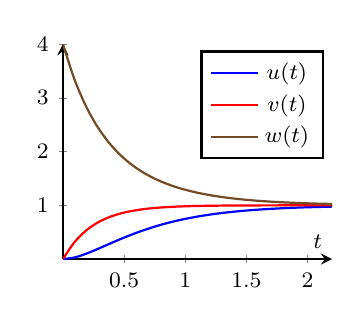
\begin{tikzpicture}
\begin{axis}[footnotesize,font=\footnotesize
,axis lines=middle,xlabel={$t$},no marks,thick
,domain=0:2.2,smooth,legend pos=north east]
\addplot+[]{1-2*exp(-2*x)+exp(-4*x)};
\addlegendentry{$u(t)$};
\addplot+[]{1-exp(-4*x)};
\addlegendentry{$v(t)$};
\addplot+[]{1+2*exp(-2*x)+exp(-4*x)};
\addlegendentry{$w(t)$};
\end{axis}
\end{tikzpicture}}%
\begin{eqnarray*}
\begin{bmatrix} u\\v\\w \end{bmatrix}
&=&\begin{bmatrix} 1\\1\\1 \end{bmatrix}
-2\begin{bmatrix} 1\\0\\-1 \end{bmatrix}e^{-2t}
-\begin{bmatrix} -1\\1\\-1 \end{bmatrix}e^{-4t}
\\&=&\begin{bmatrix} 1-2e^{-2t}+e^{-4t}\\1-e^{-4t}\\1+2e^{-2t}+e^{-4t} \end{bmatrix}.
\end{eqnarray*}
\end{solution}
\end{example}





\begin{example} \label{eg:}
Use \script\ to find a general solution to the system of differential equations
\begin{eqnarray*}
&&dx_1/dt=-\tfrac12x_1-\tfrac12x_2+x_3+2x_4\,, 
\\&&dx_2/dt=-\tfrac12x_1-\tfrac12x_2+2x_3+x_4\,, 
\\&&dx_3/dt=x_1+2x_2-\tfrac12x_3-\tfrac12x_4\,,  
\\&&dx_4/dt=2x_1+x_2-\tfrac12x_3-\tfrac12x_4\,.
\end{eqnarray*}
What is the \idx{particular solution} that satisfies the \idx{initial condition}s \(x_1(0)=-5\)\,, \(x_2(0)=-1\) and \(x_3(0)=x_4(0)=0\)\,?
Record your commands and give reasons.
%a=0+round(randn(1,4)*3),A=toeplitz(a([1 end:-1:2]),a),[v,d]=eig(A)
%P=[1 1 1 1;1 1 -1 -1;1 -1 -1 1;1 -1 1 -1]/2, A=P*diag(round(randn(1,4)*2))*P', [V,D]=eig(A)
\begin{solution} 
Write the system in matrix-vector form \(\D t\xv=A\xv\) for vector 
\begin{equation*}
\xv=\begin{bmatrix} x_1\\x_2\\x_3\\x_4 \end{bmatrix}
\quad\text{and matrix }
A=\begin{bmatrix} -\tfrac12 & -\tfrac12 & 1 & 2
\\-\tfrac12 & -\tfrac12 & 2 & 1
\\1 & 2 & -\tfrac12 & -\tfrac12
\\2 & 1 & -\tfrac12 & -\tfrac12 \end{bmatrix}.
\end{equation*}
Enter the matrix into \script\ and then find its eigenvalues and eigenvectors as follows
\begin{verbatim}
A=[-1/2 -1/2 1 2
 -1/2 -1/2 2 1
 1 2 -1/2 -1/2
 2 1 -1/2 -1/2]
[V,D]=eig(A)
\end{verbatim}
\setbox\ajrqrbox\hbox{\qrcode{% DEs
A=[-1/2 -1/2 1 2
 -1/2 -1/2 2 1
 1 2 -1/2 -1/2
 2 1 -1/2 -1/2]
[V,D]=eig(A)
c=V\slosh[-5;-1;0;0]
}}\marginpar{\usebox{\ajrqrbox}}%
\script\ tells us the eigenvectors and eigenvalues:
\begin{verbatim}
V =
  -0.5000   0.5000  -0.5000  -0.5000
  -0.5000  -0.5000   0.5000  -0.5000
   0.5000   0.5000   0.5000  -0.5000
   0.5000  -0.5000  -0.5000  -0.5000
D =
  -4.0000        0        0        0
        0  -1.0000        0        0
        0        0   1.0000        0
        0        0        0   2.0000
\end{verbatim}
Then \autoref{thm:ddtsol} gives that a general solution of the differential equations is
\begin{equation*}
\xv=
c_1\begin{bmatrix} -\tfrac12\\-\tfrac12\\\tfrac12\\\tfrac12 \end{bmatrix}e^{-4t}
+c_2\begin{bmatrix} \tfrac12\\-\tfrac12\\\tfrac12\\-\tfrac12 \end{bmatrix}e^{-t}
+c_3\begin{bmatrix} -\tfrac12\\\tfrac12\\\tfrac12\\-\tfrac12 \end{bmatrix}e^{t}
+c_4\begin{bmatrix} -\tfrac12\\-\tfrac12\\-\tfrac12\\-\tfrac12 \end{bmatrix}e^{2t}.
\end{equation*}
Given the specified initial conditions at \(t=0\)\,, when all the above exponentials reduce to \(e^0=1\)\,, we just need to find the linear combination of the eigenvectors that equals the initial vector \(\xv(0)=(-5,-1,0,0)\); that is, we solve \(V\cv=\xv(0)\).
In \script\ compute \verb|c=V\[-5;-1;0;0]| to find the vector of coefficients is \(\cv=(3,-2,2,3)\).
Hence the particular solution is
\begin{equation*}
\xv=
\begin{bmatrix} -\tfrac32\\-\tfrac32\\\tfrac32\\\tfrac32 \end{bmatrix}e^{-4t}
+\begin{bmatrix} -1\\1\\-1\\1 \end{bmatrix}e^{-t}
+\begin{bmatrix} -1\\1\\1\\-1 \end{bmatrix}e^{t}
+\begin{bmatrix} -\tfrac32\\-\tfrac32\\-\tfrac32\\-\tfrac32 \end{bmatrix}e^{2t}.
\end{equation*}
\end{solution}
\end{example}








\begin{example} \label{eg:decis2t} 
Find (by hand) a general solution to the system of differential equations
\(\D ty=z\) and \(\D tz=-4y\)\,.
\begin{solution} 
Let vector~\(\yv=(y,z)\), and then form the differential equations into the matrix-vector system
\begin{equation*}
\D t\yv=\begin{bmatrix} \D ty\\\D tz \end{bmatrix}
=\begin{bmatrix} z\\-4y \end{bmatrix}
=\begin{bmatrix} 0&1\\-4&0 \end{bmatrix}
\begin{bmatrix} y\\z \end{bmatrix}
=\underbrace{\begin{bmatrix} 0&1\\-4&0 \end{bmatrix}}_A\yv\,.
\end{equation*}
To use \autoref{thm:ddtsol} we need eigenvalues and eigenvectors of the matrix~\(A\).
Here the characteristic polynomial of~\(A\) is
\begin{equation*}
\det(A-\lambda I)=\det\begin{bmatrix} -\lambda&1\\-4&-\lambda \end{bmatrix}
=\lambda^2+4\,.
\end{equation*}
This determinant is only zero for \(\lambda^2=-4\), that is, \(\lambda=\pm2i\) (where \(i=\sqrt{-1}\))---a pair of complex conjugate eigenvalues.
\begin{itemize}
\item For eigenvalue \(\lambda=+2i\) the corresponding eigenvectors~\(\pv\) satisfy
\begin{equation*}
(A-\lambda I)\pv=\begin{bmatrix} -2i&1\\-4&-2i \end{bmatrix}\pv
=\ov.
\end{equation*}
The second row of this matrix is \(-2i\)~times the first row so we just need to satisfy the first row equation \(\begin{bmatrix} -2i&1 \end{bmatrix}\pv=0\)\,.
This equation is \(-2ip_1+p_2=0\), that is, \(p_2=2ip_1\).
Hence all eigenvectors are of the form \(\pv=(1,2i)p_1\)\,.
Choose any one, say \(\pv=(1,2i)\).

\item Similarly, for eigenvalue \(\lambda=-2i\) the corresponding eigenvectors~\(\pv\) satisfy
\begin{equation*}
(A-\lambda I)\pv=\begin{bmatrix} 2i&1\\-4&2i \end{bmatrix}\pv
=\ov.
\end{equation*}
The second row of this matrix is \(2i\)~times the first row so we just need to satisfy the first row equation \(\begin{bmatrix} 2i&1 \end{bmatrix}\pv=0\)\,.
This equation is \(2ip_1+p_2=0\), that is, \(p_2=-2ip_1\).
Hence all eigenvectors are of the form \(\pv=(1,-2i)p_1\)\,.
Choose any one, say \(\pv=(1,-2i)\).
\end{itemize}
With these two distinct eigenvalues, corresponding eigenvectors are linearly independent, and so \autoref{thm:ddtsol} gives a general solution of the differential equations as
\begin{equation*}
\begin{bmatrix} y\\z \end{bmatrix}
=c_1\begin{bmatrix} 1\\2i \end{bmatrix}e^{i2t}
+c_2\begin{bmatrix} 1\\-2i \end{bmatrix}e^{-i2t}.
\end{equation*}
That is, \(y(t)=c_1e^{i2t}+c_2e^{-i2t}\) and \(z(t)=2ic_1e^{i2t}-2ic_2e^{-i2t}\) for every constants~\(c_1\) and~\(c_2\).
These formulas answer the exercise.
The next examples show that because of the complex exponentials, this solution describes oscillations in time~\(t\).
\end{solution}
\end{example}




\begin{example} \label{eg:decis2tb} 
Further consider \autoref{eg:decis2t}.
Suppose we additionally know that \(y(0)=3\) and \(z(0)=0\)\,.  
Find the \idx{particular solution} that satisfies these two \idx{initial condition}s.
\begin{solution} 
Use the derived general solution that \(y(t)=c_1e^{i2t}+c_2e^{-i2t}\) and \(z(t)=2ic_1e^{i2t}-2ic_2e^{-i2t}\).
We find the constants~\(c_1\) and~\(c_2\) so that these satisfy the  conditions \(y(0)=3\) and \(z(0)=0\)\,.
Substitute \(t=0\) into the general solution to require, using \(e^0=1\)\,,
\begin{eqnarray*}
&&y(0)=3=c_1e^{i2\cdot0}+c_2e^{-i2\cdot0}=c_1+c_2\,,
\\&&z(0)=0=2ic_1e^{i2\cdot0}-2ic_2e^{-i2\cdot0}=2ic_1-2ic_2\,,
\end{eqnarray*}
The second of these equations requires \(2ic_1=2ic_2\)\,, that is, \(c_1=c_2\)\,.
The first, \(c_1+c_2=3\)\,, then requires that \(2c_1=3\)\,, that is, \(c_1=3/2\) and so \(c_2=3/2\)\,.
Hence the particular solution is
\begin{equation*}
y(t)=\frac32e^{i2t}+\frac32e^{-i2t} 
\quad\text{and}\quad
z(t)=3ie^{i2t}-3ie^{-i2t}.
\end{equation*}
But recall \idx{Euler's formula} that \(e^{i\theta}=\cos\theta+i\sin\theta\) for any~\(\theta\).
Invoking Euler's formula the above particular solution simplifies:
\marginpar{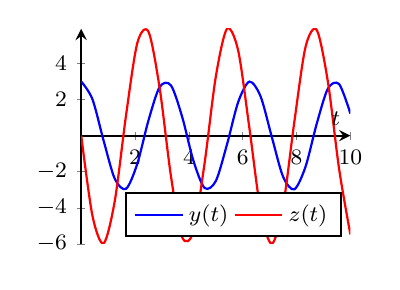
\begin{tikzpicture}
\begin{axis}[footnotesize,font=\footnotesize
,axis lines=middle,xlabel={$t$},no marks,thick
,domain=0:10,smooth,legend pos=south east,legend columns=2]
\addplot+[]{3*cos(2*deg(x))};
\addlegendentry{$y(t)$};
\addplot+[]{-6*sin(2*deg(x))};
\addlegendentry{$z(t)$};
\end{axis}
\end{tikzpicture}}%
\begin{eqnarray*}
y(t)&=&\frac32[\cos2t+i\sin2t]+\frac32[\cos(-2t)+i\sin(-2t)]
\\&=&\frac32\cos2t+\frac32i\sin2t+\frac32\cos2t-\frac32i\sin2t
\\&=&3\cos2t\,,
\\z(t)&=&3i[\cos2t+i\sin2t]-3i[\cos(-2t)+i\sin(-2t)]
\\&=&3i\cos2t-3\sin2t-3i\cos2t-3\sin2t
\\&=&-6\sin2t\,.
\end{eqnarray*}
Because \(y(t)\) and~\(z(t)\) are just trigonometric functions of~\(t\), they oscillate in time~\(t\), as illustrated in the margin.
\end{solution}
\end{example}



\begin{example} \label{eg:realcis}
In a real application the complex numbers of the general solution to \autoref{eg:decis2t} are usually inconvenient.  
Instead we often express the solution solely in terms of real quantities as just done in the previous \autoref{eg:decis2tb}.
Use \idx{Euler's formula}, that \(e^{i\theta}=\cos\theta+i\sin\theta\) for any~\(\theta\), to rewrite the general solution of \autoref{eg:decis2t} in terms of real functions.
\begin{solution}
Here use Euler's formula in the expression for
\begin{eqnarray*}
y(t)&=&c_1e^{i2t}+c_2e^{-i2t}
\\&=&c_1[\cos 2t+i\sin2t]+c_2[\cos(-2t)+i\sin(-2t)]
\\&=&c_1\cos2t+ic_1\sin2t +c_2\cos2t-ic_2\sin2t
\\&=&(c_1+c_2)\cos2t +(ic_1-ic_2)\sin2t
\\&=&C_1\cos2t+C_2\sin2t
\end{eqnarray*}
for constants \(C_1=c_1+c_2\) and \(C_2=i(c_1-c_2)\).
Let's view the arbitrariness in~\(c_1\) and~\(c_2\) as being `transferred' to~\(C_1\) and~\(C_2\), then \(y(t)=C_1\cos2t+C_2\sin2t\) is a general solution to the differential equations, and is expressed purely in real factors.
In such a real form we explicitly see the oscillations in time~\(t\) through the trigonometric functions \(\cos 2t\) and~\(\sin2t\)\,.

The function \(z(t)=2ic_1e^{i2t}-2ic_2e^{-i2t}\) has a corresponding form found by replacing~\(c_1\) and~\(c_2\) in terms of the same~\(C_1\) and~\(C_2\).
From above, the constants \(C_1=c_1+c_2\) and \(C_2=i(c_1-c_2)\).
Adding the first to \(\pm i\)~times the second determines \(C_1-iC_2=2c_1\) and \(C_1+iC_2=2c_2\)\,, so that \(c_1=(C_1-iC_2)/2\) and \(c_2=(C_1+iC_2)/2\)\,.  
Then the expression for
\begin{eqnarray*}
z(t)&=&2ic_1e^{i2t}-2ic_2e^{-i2t}
\\&=&2i\frac{C_1-iC_2}2[\cos2t+i\sin2t]
\\&&{}
-2i\frac{C_1+iC_2}2[\cos2t-i\sin2t]
\\&=&(iC_1+C_2)[\cos2t+i\sin2t]
\\&&{}
+(-iC_1+C_2)[\cos2t-i\sin2t]
\\&=&iC_1\cos2t-C_1\sin2t+C_2\cos2t+iC_2\sin2t
\\&&{}
-iC_1\cos2t-C_1\sin2t+C_2\cos2t-iC_2\sin2t
\\&=&-2C_1\sin2t+2C_2\cos2t\,.
\end{eqnarray*}
That is, the corresponding general solution \(z(t)=-2C_1\sin2t+2C_2\cos2t\) is now also expressed in real factors.
\end{solution}
\end{example}




\begin{example}[oscillating applications] \label{eg:sprmas}
\def\temp#1{\begin{tikzpicture}
\def\ugh{\ifnum0=#1 axis x line=none
\else axis x line=middle,xlabel={$x$},xtick={0}\fi}
\begin{axis}[footnotesize,font=\footnotesize
, axis y line=none,smooth,legend pos=south west
,domain=0:5.5,samples=40,axis equal,xmax=2,\ugh]
\addplot+[thick,no marks] ({2*x-cos(x*360)-12},{sin(x*360)});
\addlegendentry{spring $k$};
\addplot+[only marks,mark=*,mark size=1ex] coordinates {(0,0)};
\addlegendentry{mass $m$};
\end{axis}
\end{tikzpicture}}
A huge variety of vibrating systems are analogous to the basic oscillations of a mass on a spring, 
\marginpar{\temp0}illustrated schematically in the margin.
The mass generally will oscillate to and fro.  
Describe such a system mathematically with two differential equations, and solve the differential equations to confirm it oscillates.
\begin{solution} 
At every time~\(t\), let the position of the mass relative to its rest position be denoted by~\(x(t)\): that is, we put an \(x\)-axis on the picture with \(x=0\) where the mass would stay at rest, \marginpar{\temp1} as illustrated.
At every time~\(t\) let the mass be moving with velocity~\(v(t)\) (positive to the right, negative to the left).
Then we know one differential equation, that \(\D tx=v\).

Newton's law, that \(\text{mass}\times\text{acceleration}=\text{force}\), provides another differential equation.
Here the mass is denoted by~\(m\), and the acceleration is~\(\D tv\).
The force on the mass come from the spring: typically the force by the spring is proportional to the stretching of the spring, namely to~\(x\).
Different springs give different strength forces so let's denote the constant of proportionality by~\(k\)---a constant that differs depending upon the spring.
Then the force will be~\(-kx\) as springs try to pull\slash push the mass back towards \(x=0\)\,.
Consequently Newton's law gives us the differential equation, \(m\D tv=-kx\)\,.  
Divide by mass~\(m\) and the differential equation is \(\D tv=-\frac kmx\)\,.

Write these two differential equations together as a matrix-vector system: 
\begin{equation*}
\begin{bmatrix} \D tx\\\D tv \end{bmatrix}
=\begin{bmatrix} v\\-\frac kmx \end{bmatrix},
\quad\text{that is,}\quad
\D t{}\begin{bmatrix} x\\v \end{bmatrix}
=\begin{bmatrix} 0&1\\-\frac km&0 \end{bmatrix}\begin{bmatrix} x\\v \end{bmatrix}.
\end{equation*}
\autoref{thm:ddtsol} asserts a general solution comes from the eigenvalues and eigenvectors of the matrix.
\begin{itemize}
\item Here the characteristic polynomial of the matrix is
\begin{equation*}
\det\begin{bmatrix} -\lambda&1\\-\frac km&-\lambda \end{bmatrix}
=\lambda^2+\frac km\,.
\end{equation*}
This polynomial is zero only when the eigenvalues \(\lambda=\pm\sqrt{-k/m}=\pm i\sqrt{k/m}\)\,: these are a complex conjugate pair of pure imaginary eigenvalues.

\item  The corresponding eigenvectors~\pv\ satisfy
\begin{equation*}
\begin{bmatrix} \mp i\sqrt{k/m}&1\\- k/m&\mp i\sqrt{k/m} \end{bmatrix}
\pv=\ov.
\end{equation*}
The two rows of this equation are satisfied by the corresponding eigenvectors \(\pv\propto (1,\pm i\sqrt{k/m})\).
\end{itemize}
Then a general solution to the system of differential equations is
\begin{equation*}
\begin{bmatrix} x\\v \end{bmatrix}
=c_1\begin{bmatrix} 1\\i\sqrt{k/m} \end{bmatrix}e^{i\sqrt{k/m}t}
+c_2\begin{bmatrix} 1\\-i\sqrt{k/m} \end{bmatrix}e^{-i\sqrt{k/m}t}.
\end{equation*}
This formula shows that the mass on the spring generally oscillates as the complex exponentials are oscillatory.

However, in real applications we usually prefer a real algebraic expression.
Just as in \autoref{eg:realcis}, we make the above formula real by changing from (complex) arbitrary constants~\(c_1\) and~\(c_2\) to new (real) arbitrary constants~\(C_1\) and~\(C_2\) where \(c_1=(C_1-iC_2)/2\) and \(c_2=(C_1+iC_2)/2\).
Substitute these relations into the above general solution, and using Euler's formula, gives the position
\begin{eqnarray*}
x(t)&=&c_1e^{i\sqrt{k/m}t}+c_2e^{-i\sqrt{k/m}t}
\\&=&\frac{C_1-iC_2}2\big[\cos(\sqrt{k/m}t)+i\sin(\sqrt{k/m}t)\big]
\\&&{}
+\frac{C_1+iC_2}2\big[\cos(\sqrt{k/m}t)-i\sin(\sqrt{k/m}t)\big]
\\&=&
\frac{C_1}2\cos(\sqrt{k/m}t)+i\frac{C_1}2\sin(\sqrt{k/m}t)
\\&&{}
-i\frac{C_2}2\cos(\sqrt{k/m}t)+\frac{C_2}2\sin(\sqrt{k/m}t)
\\&&{}
+\frac{C_1}2\cos(\sqrt{k/m}t)-i\frac{C_1}2\sin(\sqrt{k/m}t)
\\&&{}
+i\frac{C_2}2\cos(\sqrt{k/m}t)+\frac{C_2}2\sin(\sqrt{k/m}t)
\\&=&C_1\cos(\sqrt{k/m}t)+C_2\sin(\sqrt{k/m}t).
\end{eqnarray*}
For all values of the arbitrary constants~\(C_1\) and~\(C_2\), this formula describes the position~\(x(t)\) of the mass as purely real oscillations in time.
Similarly for the velocity~\(v(t)\) (\autoref{ex:sprmas}).
\end{solution}
\end{example}




\index{differential equations|)}



\begin{comment}
Probable section includes Cayley--Hamilton theorem: recall \autoref{sec:mpmev}, compute powers of matrices, then C-H.
Other applications include Markov chains.

Possibly develop a little more theory on similarity of matrices and coordinate transform of matrices.  Then Jordan form and solving non-diagonalisable systems of differential equations.

Possibly something on {Emergent quasi-stationary dynamics of metastable states} but perhaps done in 7.1.2--3. (Can one have too many buzz-words?)
\end{comment}















\subsection{Exercises}


\begin{exercise} \label{ex:whichp} 
Which of the following matrices diagonalise the matrix \(Z=\begin{bmatrix} 7&12\\-2&-3 \end{bmatrix}\)?  
Show your working.
%\begin{verbatim}
%n=2
%for i=1:9999,P=0+round(randn(n)*2);if abs(det(P))==1,break,end,end
%P=P,D=diag(round(randn(1,n)*2)),A=round(P*D*inv(P))
%\end{verbatim}
\begin{parts}
\item \(P_{\alph{enumii}}=\begin{bmatrix} -2&3\\1&-1 \end{bmatrix}\)
\answer{yes}

\item \(P_{\alph{enumii}}=\begin{bmatrix} 3&-2\\-1&1 \end{bmatrix}\)
\answer{yes}

\item \(P_{\alph{enumii}}=\begin{bmatrix} 1&-1\\-2&3 \end{bmatrix}\)
\answer{no}

\item \(P_{\alph{enumii}}=\begin{bmatrix} 1&3\\1&2 \end{bmatrix}\)
\answer{no}

\item \(P_{\alph{enumii}}=\begin{bmatrix} 4&3\\-2&-1 \end{bmatrix}\)
\answer{yes}

\item \(P_{\alph{enumii}}=\begin{bmatrix} -2&3\\2&-2 \end{bmatrix}\)
\answer{no}

\item \(P_{\alph{enumii}}=\begin{bmatrix} -1&1\\3&-2 \end{bmatrix}\)
\answer{no}

\item \(P_{\alph{enumii}}=\begin{bmatrix} 3&1\\2&1 \end{bmatrix}\)
\answer{no}

\end{parts}
\end{exercise}



\begin{exercise} \label{ex:whichps} 
Redo \autoref{ex:whichp} by finding which matrices~\(P_a,\ldots,P_h\) diagonalise each of the following matrices.
\begin{parts}
\item \(\eAii=\begin{bmatrix} 5&12\\-2&-5 \end{bmatrix}\)
\item \(\eAii=\begin{bmatrix} -3&-12\\2&7 \end{bmatrix}\)
\item \(\eAii=\begin{bmatrix} -1&-1\\6&4 \end{bmatrix}\)
\item \(\eAii=\begin{bmatrix} 4&6\\-1&-1 \end{bmatrix}\)
\end{parts}
\end{exercise}




\begin{exercise} \label{ex:} 
Following \autoref{eg:diagonaliseb}, prove that the matrix \(\begin{bmatrix} k&1\\0&k \end{bmatrix}\) is not diagonalisable for every scalar~\(k\).
\end{exercise}




\begin{exercise} \label{ex:} 
In each of the following cases, you are given three linearly independent eigenvectors and corresponding eigenvalues for some \(3\times3\) matrix~\(A\).
Write down three different matrices~\(P\) that will diagonalise the matrix~\(A\), and for each write down the corresponding diagonal matrix \(D=P^{-1}AP\).
\begin{enumerate}
\item \(\lambda_1=-1\), \(\pv_1=(3,2,-1)\);
\(\lambda_2=1\), \(\pv_2=(-4,-2,2)\);
\(\lambda_3=3\), \(\pv_3=(-1,0,2)\).

\item \(\lambda_1=-1\), \(\pv_1=( 2,1,2)\);
\(\lambda_2=-1\), \(\pv_2=(0,3,1)\);
\(\lambda_3=2\), \(\pv_3=(4,-2,-2)\).

\item \(\lambda_1=1\), \(\pv_1=(3,-7,2)\);
\(\lambda_2=-2\), \(\pv_2=(-4,-5,1)\);
\(\lambda_3=4\), \(\pv_3=(1,2,3)\).

\item \(\lambda_1=3\), \(\pv_1=(2,-3,0)\);
\(\lambda_2=1\), \(\pv_2=(-1,2,-6)\);
\(\lambda_3=-4\), \(\pv_3=(-2,-1,-3)\).

\end{enumerate}
\end{exercise}





\begin{exercise} \label{ex:} 
From the given information, are each of the matrices diagonalisable?  
Give reasons.
\begin{enumerate}
\item The only eigenvalues of a \(2\times2\) matrix are \(2.2\) and~\(0.1\).
\answer{yes}

\item The only eigenvalues of a \(4\times4\) matrix are \(2.2\), \(1.9\), \(-1.8\) and~\(-1\).
\answer{yes}

\item The only eigenvalue of a \(2\times2\) matrix is~\(0.7\).
\answer{unknown}

\item The only eigenvalues of a \(6\times6\) matrix are \(-1.6\), \(0.3\), \(0.1\) and~\(-2.3\).
\answer{unknown}

\item The only eigenvalues of a \(5\times5\) matrix are \(-1.7\), \(1.4\), \(1.3\), \(2.4\), \(0.5\) and~\(-2.3\).
\answer{error}

\item The only eigenvalues of a \(6\times6\) matrix are \(1.2\), \(-0.9\), \(-0.8\), \(2.2\), \(0.2\) and~\(-0.2\).
\answer{yes}

\item The \script\ function \verb|eig(A)| returns the result
\begin{verbatim}
ans =
   2.6816
  -0.1445
   0.0798
   0.3844
\end{verbatim}
\answer{yes}

\item The \script\ function \verb|eig(A)| returns the result
\begin{verbatim}
ans =
   3.0821 + 0.0000i
  -2.7996 + 0.0000i
  -0.7429 + 1.6123i
  -0.7429 - 1.6123i
\end{verbatim}
\answer{yes}

\item The \script\ function \verb|eig(A)| returns the result
\begin{verbatim}
ans =
  -1.0000
   1.0000
   2.0000
  -1.0000
\end{verbatim}
\answer{unknown}

\end{enumerate}
\end{exercise}




\begin{exercise} \label{ex:} 
For each of the following \(3\times3\) matrices, show with hand algebra that each matrix has one eigenvalue of multiplicity three, and then determine the \idx{dimension} of the corresponding \idx{eigenspace}.
Also compute the eigenvalue and eigenvectors with \script: comment on any limitations in the computed `eigenvalues' and `eigenvectors'.
%\begin{verbatim}
%d=eye(3)*round(randn)+[0 round(rand) 0;0 0 round(rand); 0 0 0], for i=1:99999,p=round(randn(3)*3); if abs(det(p))==1, a=round(p*d*inv(p))+0, break, end, end, [v,d]=eig(a)
%\end{verbatim}
\begin{parts}
\item \(\eAii=\begin{bmatrix} 2 & 0 & 0
\\0 & 2 & 0
\\0 & 0 & 2 \end{bmatrix}\)
\answer{\(\lambda=2\), three; all good}

\item \(\eAii=\begin{bmatrix} 2 & 1 & -2
\\-8 & -4 & 8
\\-2 & -1 & 2 \end{bmatrix}\)
\answer{\(\lambda=0\), two; errors~\(10^{-8}\) and two  eigenvectors effectively the same.}

\item \(\eAii=\begin{bmatrix} -2 & 1 & 0
\\0 & -2 & 0
\\0 & 1 & -2 \end{bmatrix}\)
\answer{\(\lambda=-2\), two; not lin.~indep.}

\item \(\eAii=\begin{bmatrix} 7 & 1 & 22
\\-6 & -1 & -20
\\-1 & 0 & -3 \end{bmatrix}\)
\answer{\(\lambda=1\), one; errors~\(10^{-5}\), all three eigenvectors effectively the same}

\item \(\eAii=\begin{bmatrix} 3 & 5 & -1
\\-4 & -6 & 1
\\-5 & -6 & 0 \end{bmatrix}\)
\answer{\(\lambda=-1\), one; errors~\(10^{-6}\), all three eigenvectors \(\pm\)same}

\item \(\eAii=\begin{bmatrix} -6 & -5 & 3
\\-4 & -7 & 3
\\-12 & -15 & 7 \end{bmatrix}\)
\answer{\(\lambda=0\), two; errors~\(10^{-8}\) and two  eigenvectors effectively the same.}

\item \(\eAii=\begin{bmatrix} -3 & 2 & 7
\\2 & -3 & -9
\\-1 & 1 & 3 \end{bmatrix}\)
\answer{\(\lambda=-1\), one;  errors~\(10^{-6}\), all three eigenvectors \(\pm\)same}

\item \(\eAii=\begin{bmatrix} -1 & 0 & 0
\\0 & -1 & 0
\\0 & 0 & -1 \end{bmatrix}\)
\answer{\(\lambda=-1\), three; all good}


\end{parts}
\end{exercise}







\begin{exercise} \label{ex:dimme} 
For a given \(n\times n\) square matrix~\(A\), suppose \(\lambda_1\) is an eigenvalue with \(n\)~corresponding linearly independent eigenvectors \hlist\pv n\,.  
Adapt parts of the proof of \autoref{thm:dimee} to prove that the \idx{characteristic polynomial} of matrix~\(A\) is \(\det(A-\lambda I)=(\lambda_1-\lambda)^n\). 
Then deduce that \(\lambda_1\)~is the only eigenvalue of~\(A\), and is of multiplicity~\(n\).
\end{exercise}




\begin{exercise} \label{ex:} 
For each of the following matrices, use \script\ to find the eigenvalues, their \idx{multiplicity}, and the dimension of the \idx{eigenspace}s.  Give reasons (remember computational error).
%\begin{verbatim}
%d=0+round(randn(1,2)*2);
%d=diag([d(1) d(1) d(1) d(2) d(2)]);
%d([2 6 8 12 20 24])=0+round(rand(6,1)*0.75).*[-1;1;-1;1;-1;1]
%for i=1:99999,p=round(randn(5)*3); if min(abs(abs(det(p))-[1 2 5]))<1e-7, a=p*d*inv(p), break, end, end,[V,D]=eig(a)
%\end{verbatim}
\begin{enumerate}
\item \(\eAii=\begin{bmatrix} -30.5 & 25.5 & 22 & -5 & -48.5
\\-111 & 88 & 76 & -20 & -173
\\87.5 & -70.5 & -61 & 16 & 136.5
\\51 & -43 & -36 & 9 & 81
\\-4.5 & 2.5 & 2 & -1 & -6.5 \end{bmatrix}\)
\setbox\ajrqrbox\hbox{\qrcode{% eig
A=[-30.5 25.5 22 -5 -48.5
 -111 88 76 -20 -173
 87.5 -70.5 -61 16 136.5
 51 -43 -36 9 81
 -4.5 2.5 2 -1 -6.5]
}}\marginpar{\usebox{\ajrqrbox}}%
\answer{\(\lambda=1\) twice, \(\dim\EE_{1}=1\); \(\lambda=-1\) thrice, \(\dim\EE_{-1}=2\)}

\item \(\eAii=\begin{bmatrix} 2929 & 1140 & -1359 & 2352 & 406
\\-2441 & -950 & 1132 & -1960 & -338
\\-1070 & -416 & 495 & -858 & -148
\\-2929 & -1140 & 1359 & -2352 & -406
\\-895 & -347 & 412 & -715 & -124 \end{bmatrix}\)
\setbox\ajrqrbox\hbox{\qrcode{% eig
A=[2929 1140 -1359 2352 406
 -2441 -950 1132 -1960 -338
 -1070 -416 495 -858 -148
 -2929 -1140 1359 -2352 -406
 -895 -347 412 -715 -124]
}}\marginpar{\usebox{\ajrqrbox}}%
\answer{\(\lambda=-1\) twice, \(\dim\EE_{-1}=1\); \(\lambda=0\) thrice, \(\dim\EE_{0}=2\)}

\item \(\eAii=\begin{bmatrix} -168 & 115 & 305 & -120 & 70
\\-4710 & 3202 & 8510 & -3360 & 1990
\\450 & -305 & -813 & 320 & -190
\\-4545 & 3090 & 8205 & -3243 & 1920
\\-2415 & 1640 & 4355 & -1720 & 1017 \end{bmatrix}\)
\setbox\ajrqrbox\hbox{\qrcode{% eig
A=[-168 115 305 -120 70
 -4710 3202 8510 -3360 1990
 450 -305 -813 320 -190
 -4545 3090 8205 -3243 1920
 -2415 1640 4355 -1720 1017]
}}\marginpar{\usebox{\ajrqrbox}}%
\answer{\(\lambda=2\) twice, \(\dim\EE_{2}=2\); \(\lambda=-3\) thrice, \(\dim\EE_{-3}=3\)}

\item \(\eAii=\begin{bmatrix} -8 & 744 & -564 & 270 & 321
\\1 & -43 & 33 & -15 & -19
\\1 & 29 & -21 & 12 & 12
\\5 & -431 & 327 & -156 & -186
\\-5 & 535 & -405 & 195 & 231 \end{bmatrix}\)
\setbox\ajrqrbox\hbox{\qrcode{% eig
A=[-8 744 -564 270 321
 1 -43 33 -15 -19
 1 29 -21 12 12
 5 -431 327 -156 -186
 -5 535 -405 195 231]
}}\marginpar{\usebox{\ajrqrbox}}%
\answer{\(\lambda=0\) twice, \(\dim\EE_{0}=2\); \(\lambda=1\) thrice, \(\dim\EE_{1}=2\)}

\item \(\eAii=\begin{bmatrix}15.6 & 31.4 & -11.6 & -14.6 & -10.6
\\-16.6 & -32.4 & 11.6 & 14.6 & 10.6
\\33.6 & 56.4 & -19.6 & -27.6 & -15.6
\\38.6 & 75.4 & -28.6 & -35.6 & -26.6
\\-122 & -226 & 82 & 106 & 73 \end{bmatrix}\)
\setbox\ajrqrbox\hbox{\qrcode{% eig
A=[15.6 31.4 -11.6 -14.6 -10.6
 -16.6 -32.4 11.6 14.6 10.6
 33.6 56.4 -19.6 -27.6 -15.6
 38.6 75.4 -28.6 -35.6 -26.6
 -122 -226 82 106 73]
}}\marginpar{\usebox{\ajrqrbox}}%
\answer{\(\lambda=2\) twice, \(\dim\EE_{2}=1\); \(\lambda=-1\) thrice, \(\dim\EE_{-1}=3\)}

\item \(\eAii=\begin{bmatrix}-208 & 420 & -518 & 82 & 264
\\655 & -1336 & 1642 & -260 & -838
\\229 & -467 & 574 & -91 & -294
\\-171 & 348 & -428 & 66 & 218
\\-703 & 1431 & -1760 & 279 & 896 \end{bmatrix}\)
\setbox\ajrqrbox\hbox{\qrcode{% eig
A=[-208 420 -518 82 264
 655 -1336 1642 -260 -838
 229 -467 574 -91 -294
 -171 348 -428 66 218
 -703 1431 -1760 279 896]
}}\marginpar{\usebox{\ajrqrbox}}%
\answer{\(\lambda=-1\pm i\) once each, \(\dim\EE_{-1\pm i}=1\); \(\lambda=-2\) thrice, \(\dim\EE_{-2}=2\)}

\end{enumerate}
\end{exercise}






\begin{exercise} \label{ex:} 
For each of the following systems of differential equations, find eigenvalues and eigenvectors to derive a \idx{general solution} of the system of differential equations.  Show your working.
%\begin{verbatim}
%n=3,d=diag(0+round(randn(1,n)*(5-n)));for i=1:99999,p=round(randn(n)*3); if min(abs(abs(det(p))-[1 2 5 10]))<1e-7, a=round(p*d*inv(p)*100)/100, break, end, end,[V,D]=eig(a),V*diag(1./max(abs(V)))
%\end{verbatim}

\begin{parts}
\item \(\D tx=x-1.5y\), \(\D ty=4x-4y\)
\answer{\((x,y)=c_1(3,4)e^{-t}+c_2(1,2)e^{-2t}\)}

\item \(\D tx=x\), \(\D ty=-12x+5y\)
\answer{\((x,y)=c_1(0,1)e^{5t}+c_2(1,3)e^{t}\)}

\item \(\D tx=7x-3y\)
\answer{Not possible: only one equation for two unknowns.}

\item \(\D tu=2.8u-3.6v\), \(\D tv=-0.6u+2.2v\)
\answer{\((u,v)=c_1(3,-1)e^{4t}+c_2(2,1)e^{t}\)}

\item \(\D tp=14p+16q\), \(\D tq=-8p-10q\)
\answer{\((p,q)=c_1(2,-1)e^{6t}+c_2(-1,1)e^{-2t}\)}

\item \(\D tx=6.5x-0.6y-5.7z\), \(\D ty=-3x+4.4y+7.8z\)%, \(\D tz=1.5x-4.2y-7.9z\)
\answer{Not possible: only two equations for three unknowns.}

\item \(\D tx=-31x+26y-24z\), \(\D ty=-48x+39y-36z\), \(\D tz=-14x+10y-9z\)
\answer{\((x,y,z)=c_1(3,3,-1)e^{3t}+c_2(1,2,1)e^{-3t}+c_3(1,3,2)e^{-t}\)}

\item \(\D tx=0.2x+1.2z\), \(\D ty=-x\), \(\D tz=1.8x+0.8z\)
\answer{\((x,y,z)=c_1(0,1,0) +c_2(1,1,-1)e^{-t} +c_3(-2,1,3)e^{2t}\)}

\item \(\D tu=4.5u+7.5v+7.5w\), \(\D tv=3u+4v+5w\), \(\D tw=-7.5u-11.5v-12.5w\)
\answer{\((u,v,w)=c_1(-1,-1,2)e^{-3t} +c_2(-5,0,3) +c_3(0,1,-1)e^{-t}\)}

\item \(\D tp=-13p+30q+6r\), \(\D tq=-32p+69q+14r\), \(\D tr=125p-265q-54r\)
\answer{\((p,q,r)=c_1(2,2,-5)e^{2t}+c_2(3,1,2)e^{t}+c_3(0,-1,5)e^{-t}\)}

\end{parts}
\end{exercise}





\begin{exercise} \label{ex:} 
In each of the following, a general solution to a differential equation is given.  
Find the \idx{particular solution} that satisfies the specified \idx{initial condition}s.
Show your working.
\begin{enumerate}
\item \((x,y)=c_1(0,1)e^{-t}+c_2(1,3)e^{2t}\) where \(x(0)=2\) and \(y(0)=1\)
\answer{\((x,y)=-5(0,1)e^{-t}+2(1,3)e^{2t}\)}

\item \((x,y)=c_1(0,1)e^{-2t}+c_2(1,3)e^{t}\) where \(x(0)=0\) and \(y(0)=2\)
\answer{\((x,y)=(0,2)e^{-2t}\)}

\item \(x=3c_1e^t+c_2e^{-t}\), \(y=5c_1e^t+2c_2e^{-t}\) where \(x(0)=0\) and \(y(0)=2\)
\answer{\(x=-6e^t+6e^{-t}\), \(y=-10e^t+12e^{-t}\)}

\item \(x=3c_1e^t+c_2e^{2t}\), \(y=5c_1e^t+2c_2e^{2t}\) where \(x(0)=1\) and \(y(0)=3\)
\answer{\(x=-3e^t+4e^{2t}\), \(y=-5e^t+8e^{2t}\)}

\item \((x,y,z)=c_1(0,0,1) +c_2(1,-1,1)e^{2t} +c_3(-2,3,1)e^{-2t}\) where \(x(0)=3\), \(y(0)=-4\) and \(z(0)=0\)
\answer{\((x,y,z)=(1,-1,1)e^{2t} +(2,-3,-1)e^{-2t}\)}

\item \((x,y,z)=c_1(0,0,1)e^{-3t} +c_2(1,-1,1) +c_3(-2,3,1)e^{-t}\) where \(x(0)=3\), \(y(0)=-4\) and \(z(0)=2\)
\answer{\((x,y,z)=(0,0,2)e^{-3t} +(1,-1,1) +(2,-3,-1)e^{-t}\)}

\end{enumerate}
\end{exercise}







\begin{exercise} \label{ex:} 
For each of the following systems of differential equations, use \script\ to find eigenvalues and eigenvectors and hence derive a \idx{general solution} of the system of differential equations.  
Record your working.
%\begin{verbatim}
%n=4,d=diag(0+round(randn(1,n)*10)/10); if rand<0.5,d(1:2,1:2)=[d(1) -d(2,2);d(2,2) d(1)],end,
%for i=1:99999,p=round(randn(n)*3); if min(abs(abs(det(p))-[1]))<1e-7, a=round(p*d*inv(p)*1e4)/1e4, break, end, end,
%[V,D]=eig(a),vd=num2str(V',2),dd=num2str(D',2)
%\end{verbatim}

\begin{enumerate}
\item \(\begin{array}{l} 
\D t{x_1}= 15.8x_1 +17.1x_2 -119.7x_3 +153.9x_4\,,\\
\D t{x_2}= 1.4x_1 +0.1x_2 +12.9x_3 -17.1x_4\,,\\
\D t{x_3}= 6.2x_1 +6.2x_2 -43x_3 +57.6x_4\,,\\
\D t{x_4}= 3.4x_1 +3.4x_2 -25x_3 +34x_4\,.
\end{array}\)
\setbox\ajrqrbox\hbox{\qrcode{% DE
A=[15.8 17.1 -119.7 153.9
 1.4 0.1 12.9 -17.1
 6.2 6.2 -43.0 57.6
 3.4 3.4 -25.0 34.0 ]
}}\marginpar{\usebox{\ajrqrbox}}%
\answer{\twodp\ \(\xv
=c_1(0.71,-0.71,0,0)e^{-1.3t} 
+c_2(-0.63,-0.63,-0.42,-0.21)e^{4.4t} 
+c_3(0,0.64,0.64,0.43)e^{1.6t} 
+c_4(-0.82,0.41,0.41)e^{2.2t}\)}

\item \(\begin{array}{l} 
\D t{x_1}= -12.2x_1 +53.7x_2 +50.1x_3 -22.8x_4\,,\\
\D t{x_2}= 0.6x_1 -2.3x_2 -2.7x_3 +1.2x_4\,,\\
\D t{x_3}= -20.4x_1 +93.8x_2 +90.2x_3 -40.8x_4\,,\\
\D t{x_4}= -38.2x_1 +177.9x_2 +170.7x_3 -77.2x_4\,.
\end{array}\)
\setbox\ajrqrbox\hbox{\qrcode{% DE
A=[ -12.2 53.7 50.1 -22.8
 0.6 -2.3 -2.7 1.2
 -20.4 93.8 90.2 -40.8
 -38.2 177.9 170.7 -77.2 ]
}}\marginpar{\usebox{\ajrqrbox}}%
\answer{\twodp\ \(\xv
=c_1(0.63,0.63,-0.42,0.21)e^{0.5t} 
+c_2(-0.23,-0.23,-0.23,-0.92)e^{0.4t} 
+c_3(0.64,0,0.43,0.64)e^{-1.6t} 
+c_4(-0.89,0,0,0.45)e^{0.8t}\)}

\item \(\begin{array}{l} 
\D t{x_1}= x_1 +29.4x_2 -3.2x_3 -12.9x_4\,,\\
\D t{x_2}= 1.4x_1 -38.4x_2 +5.6x_3 +18.2x_4\,,\\
\D t{x_3}= 2.3x_1 -80.3x_2 +12.3x_3 +36.7x_4\,,\\
\D t{x_4}= 2.4x_1 -65x_2 +9.2x_3 +31.1x_4\,.
\end{array}\)
\setbox\ajrqrbox\hbox{\qrcode{% DE
A=[ 1.0 29.4 -3.2 -12.9
 1.4 -38.4 5.6 18.2
 2.3 -80.3 12.3 36.7
 2.4 -65.0 9.2 31.1 ]
}}\marginpar{\usebox{\ajrqrbox}}%
\answer{\twodp\ \(\xv
=c_1(-0.63,0.32,0.32,0.63)e^{0.8t} 
+c_2(0.8,0.27,0,0.53)e^{2.2t} 
+c_3(0.76,0,-0.49-0.4i,0.091+0.12i)e^{(1.5-0.4i)t} 
+c_4(0.76,0,-0.49+0.4i,0.091-0.12i)e^{(1.5+0.4i)t}\)}

\item \(\begin{array}{l}
\D t{x_1}= -50.2x_1 -39.5x_2 -20.2x_3 +68.9x_4\,,\\
\D t{x_2}= 62.8x_1 +50.2x_2 +28.4x_3 -85.2x_4\,,\\
\D t{x_3}= -17.3x_1 -13.7x_2 -8.9x_3 +22.7x_4\,,\\
\D t{x_4}= -6.4x_1 -4.6x_2 -1.4x_3 +9x_4\,.
\end{array}\)
\setbox\ajrqrbox\hbox{\qrcode{% DE
A=[-50.2 -39.5 -20.2 68.9
 62.8 50.2 28.4 -85.2
 -17.3 -13.7 -8.9 22.7
 -6.4 -4.6 -1.4 9 ]
}}\marginpar{\usebox{\ajrqrbox}}%
\answer{\twodp\ \(\xv
=c_1(-0.78,0.38+0.3i,0.095+0.076i,-0.32+0.21i)e^{(0.1-1.1i)t} 
+c_2(-0.78,0.38-0.3i,0.095-0.076i,-0.32-0.21i)e^{(0.1+1.1i)t} 
+c_3(0,-0.87,0.22,-0.44)e^{0.5t} 
+c_4(-0.5,-0.5,0.5,-0.5)e^{-0.6t}\)}

\end{enumerate}
\end{exercise}





\begin{exercise} \label{ex:sprmas} 
Recall the general complex solution that \autoref{eg:sprmas} derives for the oscillations of a mass on a spring.
Show that substituting \(c_1=(C_1-iC_2)/2\) and \(c_2=(C_1+iC_2)/2\) for real~\(C_1\) and~\(C_2\) results in the velocity~\(v(t)\) being expressed algebraically in purely real terms.
\end{exercise}






\begin{comment}
Add exercises on perhaps simple SIR models, and perhaps mechanical models.

%{ED498555.pdf}
why, what caused X?
how did X occur?
what-if? what-if-not?
how does X compare with Y?
what is the evidence for X?
why is X important?
\end{comment}



\index{diagonalisation|)}

